% Created 2026-05-10 Sun 22:52
% Intended LaTeX compiler: pdflatex
\documentclass[12pt]{article}

\usepackage[utf8]{inputenc}
\usepackage[T1]{fontenc}
\usepackage{graphicx}
\usepackage{longtable}
\usepackage{wrapfig}
\usepackage{rotating}
\usepackage[normalem]{ulem}
\usepackage{amsmath}
\usepackage{amssymb}
\usepackage{capt-of}
\usepackage{hyperref}
\usepackage[singlelinecheck=false]{caption}
\usepackage{enumitem}
\usepackage{setspace}
% \onehalfspacing
% \usepackage[inner=1.0in, outer=1.0in, top=1.0in, bottom=1.0in]{geometry}
\hypersetup{
colorlinks = true,
linkcolor = blue,
filecolor = magenta,
urlcolor = cyan,
citecolor = blue
}

\usepackage{tikz}

% datasummary tables formatting
\usepackage{float}
\usepackage[normalem]{ulem}
\usepackage{tabularray}
\UseTblrLibrary{booktabs}
\UseTblrLibrary{siunitx}
\newcommand{\tinytableTabularrayUnderline}[1]{\underline{#1}}
\newcommand{\tinytableTabularrayStrikeout}[1]{\sout{#1}}
\NewTableCommand{\tinytableDefineColor}[3]{\definecolor{#1}{#2}{#3}}

% for rotating tables
\usepackage{pdflscape}
\usepackage{afterpage}

\usepackage{adjustbox}

\setcounter{secnumdepth}{3}

\author{Dante Yasui}
\date{\today}
\title{Forced Removal or Moved to Opportunity?\\\medskip
\large Labor Market and Migration Effects of Japanese Internment}
\hypersetup{
 pdfauthor={Dante Yasui},
 pdftitle={Forced Removal or Moved to Opportunity?},
 pdfkeywords={},
 pdfsubject={},
 pdfcreator={},
 pdflang={English}}
\usepackage{natbib}
\begin{document}

\maketitle
\begin{abstract}
% Intro sentence
During World War II a large scale forced migration of over 100,000
Japanese American immigrants and their citizen children
lead to relocation away from the West Coast.
% Methods
I analyse the effect that this forced relocation had
on the post-war earnings of a linked sample of likely internees.
My empirical strategy uses an individual-level panel of Japanese
and Chinese men and women to compare earnings before and after internment.
% Results
I find that individuals who were likely interned experienced faster growth in
earnings compared to their counterfactual earnings if they had not been
interned.
% Mechanisms
The possible mechaisms which might explain this seeming adaptation
include occupational change and later migration decisions.
\end{abstract}
\section{Introduction}
\label{sec:org0655be0}

The forced internment of over 120,000 Japanese Americans during World War II
stands as a stark episode of racial injustice and economic loss.
The policy displaced individuals and families
from their homes, businesses, and farms on the West Coast;
a forced displacement that fractured communities and interrupted lives.
Conventional understanding rightly frames this event as a traumatic scar,
with research documenting its detrimental effects
on property, wealth, and psychological well-being
\citep{commissiononwartimerelocationPersonalJusticeDenied1983}.

However, an emerging body of economic literature
presents a more complex and surprising picture.
Despite losses of property, job opportunities, and livelihoods,
some evidence suggests that for a subset of the internee population
this forced displacement paradoxically led to upward economic mobility
in the decades following the war
\citep{arellano-boverDisplacementDiversityMobility2022,shoagCausalEffectPlace2016}.
This finding presents a central puzzle:
How could a policy of forced removal and incarceration
have created economic \emph{opportunity}?
In this paper I examine the mechanisms through which
internment reshaped the labor market outcomes of Japanese Americans
and, crucially, for whom these effects were most pronounced.

I argue that, at least for some internees,
internment acted as a large-scale, ``move to opportunity'' experiment.
Forced relocation may have generated economic gains through two primary channels.
First, it allowed internees to escape discrimination on the West Coast,
where the anti-Japanese sentiment that originally contributed to internment
may have held back their potential post-war earnings.
Second, the quasi-random placement of internees in camps across the interior U.S.
inadvertently moved them closer to burgeoning post-war economies,
such as those in the Midwest and Chicago,
creating new labor market prospects that would have otherwise been inaccessible
\citep{austinEastwardPioneersJapanese2007}.

To test this hypothesis,
I use newly available linked census data from IPUMS
to track individuals from 1940 to 1950.
I combine these census records with detailed War Relocation Authority (WRA)
records on internee origins and camp assignments.
My empirical strategy leverages the intensity of internment at the county level
to identify its causal impact.
By comparing the outcomes of Japanese Americans
from counties with high internment rates to a control group of Chinese Americans
and non-West Coast Japanese\footnote{Those living in the US mainland outside of Arizona, California, Oregon, or Washington during 1940.}
who were not targeted by the policy,
I can estimate the effect of forced displacement on post-war earnings
and migration.

My analysis yields three key findings.
First,
greater internment exposure predicts higher 1950 earnings,
consistent with a place-based opportunity effect.
Second, this effect was not uniform across the population;
it was driven almost entirely by women.
Japanese American women who were likely internees
saw substantially larger wage gains than their non-interned peers.
This result highlights a critical intersection between forced migration
and gender dynamics.
Third, I find that these gains are linked to migration;
internees were more likely to move to
more densely populated counties with higher median incomes.

This paper contributes in three main ways.
First, it adds supporting evidence to the long-term economic consequences
of Japanese internment
and clarifies potential mechanisms behind
the surprising positive effects for labor market outcomes
found in the economic literature.

Second, this study leverages newly linked historical panel data
to study large-scale displacements of an ethnic minority group.

Third, it contributes to the broader place-effects literature
by showing how a large, exogenous shock to an individual's location
can alter their economic trajectory,
particularly for historically marginalized groups.
The findings shed light on the complex legacy of internment
and the different ways in which marginalized people can adapt
in spite of discrimination and adversity.
Importantly, the findings of this paper should not be seen
as diminishing the moral and material harms of internment overall.
My dataset does not measure property losses,
or emotional trauma from unseating an entire population from their homes.
Instead, this paper shows that despite all of these losses,
internees were able to adapt in a relatively short period of time
to the new locations and opportunities
in which they found themselves after their release.
\subsection{Historical Background}
\label{sec:orge28ed0c}

\subsubsection{Patterns of Japanese Settlement}
\label{sec:org729d912}

\subsubsection{Executive Order 9066 and the War Relocation Authority}
\label{sec:org54f0141}
\href{https://www.archives.gov/milestone-documents/executive-order-9066}{Executive Order 9066}
was signed on February 19, 1942 and granted the Secretary of War the authority
to designate military areas from which civilians could be prevented access. This
order was used to target all persons of Japanese descent living in the so-called
`Exclusion Zone' which included all of California, and large areas of
Washington, Oregon, and Arizona shown in blue in Figure \ref{fig:internmentmap}.
At first, the Secretary of War Henry Stimson encouraged some families
to relocate voluntarily from the West Coast,
but starting at the end of March 1942,
the Wartime Civil Control Administration (WCCA) and War Relocation Authority (WRA)
were established to remove all remaining Japanese Americans to temporary
Assembly Centers which were makeshift shelters in close proximity to the
population centers where these people were living. As the more permanent WRA
Relocation Centers were completed in May 1942, all Japanese Americans left
on the West Coast were moved from Assembly Centers to Relocation Centers by
train. This process lasted until November of 1942
\citep{commissiononwartimerelocationPersonalJusticeDenied1983,denshoencyclopediacontributorsResettlementDenshoEncyclopedia2020}.

As seen in Figure \ref{fig:1940JAmap}, over 90\% of the 1940 Japanese American
population lived in areas which would become subject to relocation orders.
This population was overwhelmingly concentrated along the West Coast,
particularly in California,
which was home to large, well-established Japanese American communities,
many of whom were engaged in farming and small businesses.
The geographic concentration of this population
in economically vital areas near major cities and military installations
heightened the perceived security threat,
prompting their forced relocation.

Even in the West Coast states which were subject to internment,
there was a large amount of variation in the proportion of internees
out of each county's pre-existing Japanese population
as measured in the 1940 full-count census data.

Figure \ref{fig:intern_map} shows a map of all 1940 counties
shaded by the proportion of WRA internees from that county
out of the 1940 Japanese population.
Counties in dark blue had Japanese residents in 1940,
but none appear in the internment records.
Counties in yellow had as many (or more) of their 1940 Japanese residents
appear in the WRA records as internees.
Counties that are not shaded did not have any 1940 Japanese residents.

\begin{figure}
  \caption{\label{fig:intern_map} Proportion of 1940 Japanese population interned}
  \begin{adjustbox}{width=\textwidth, center}
    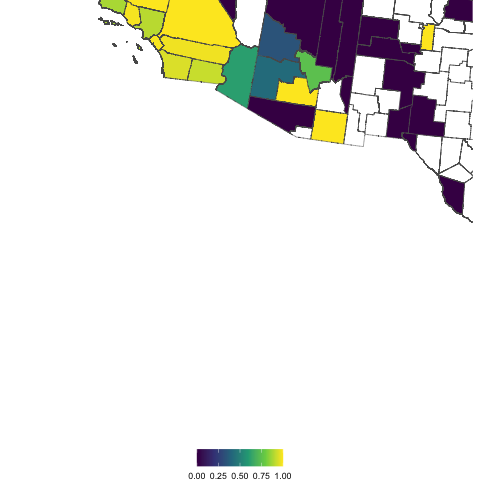
\includegraphics[width=\textwidth]{../figures/pr_interned_map.png}
  % 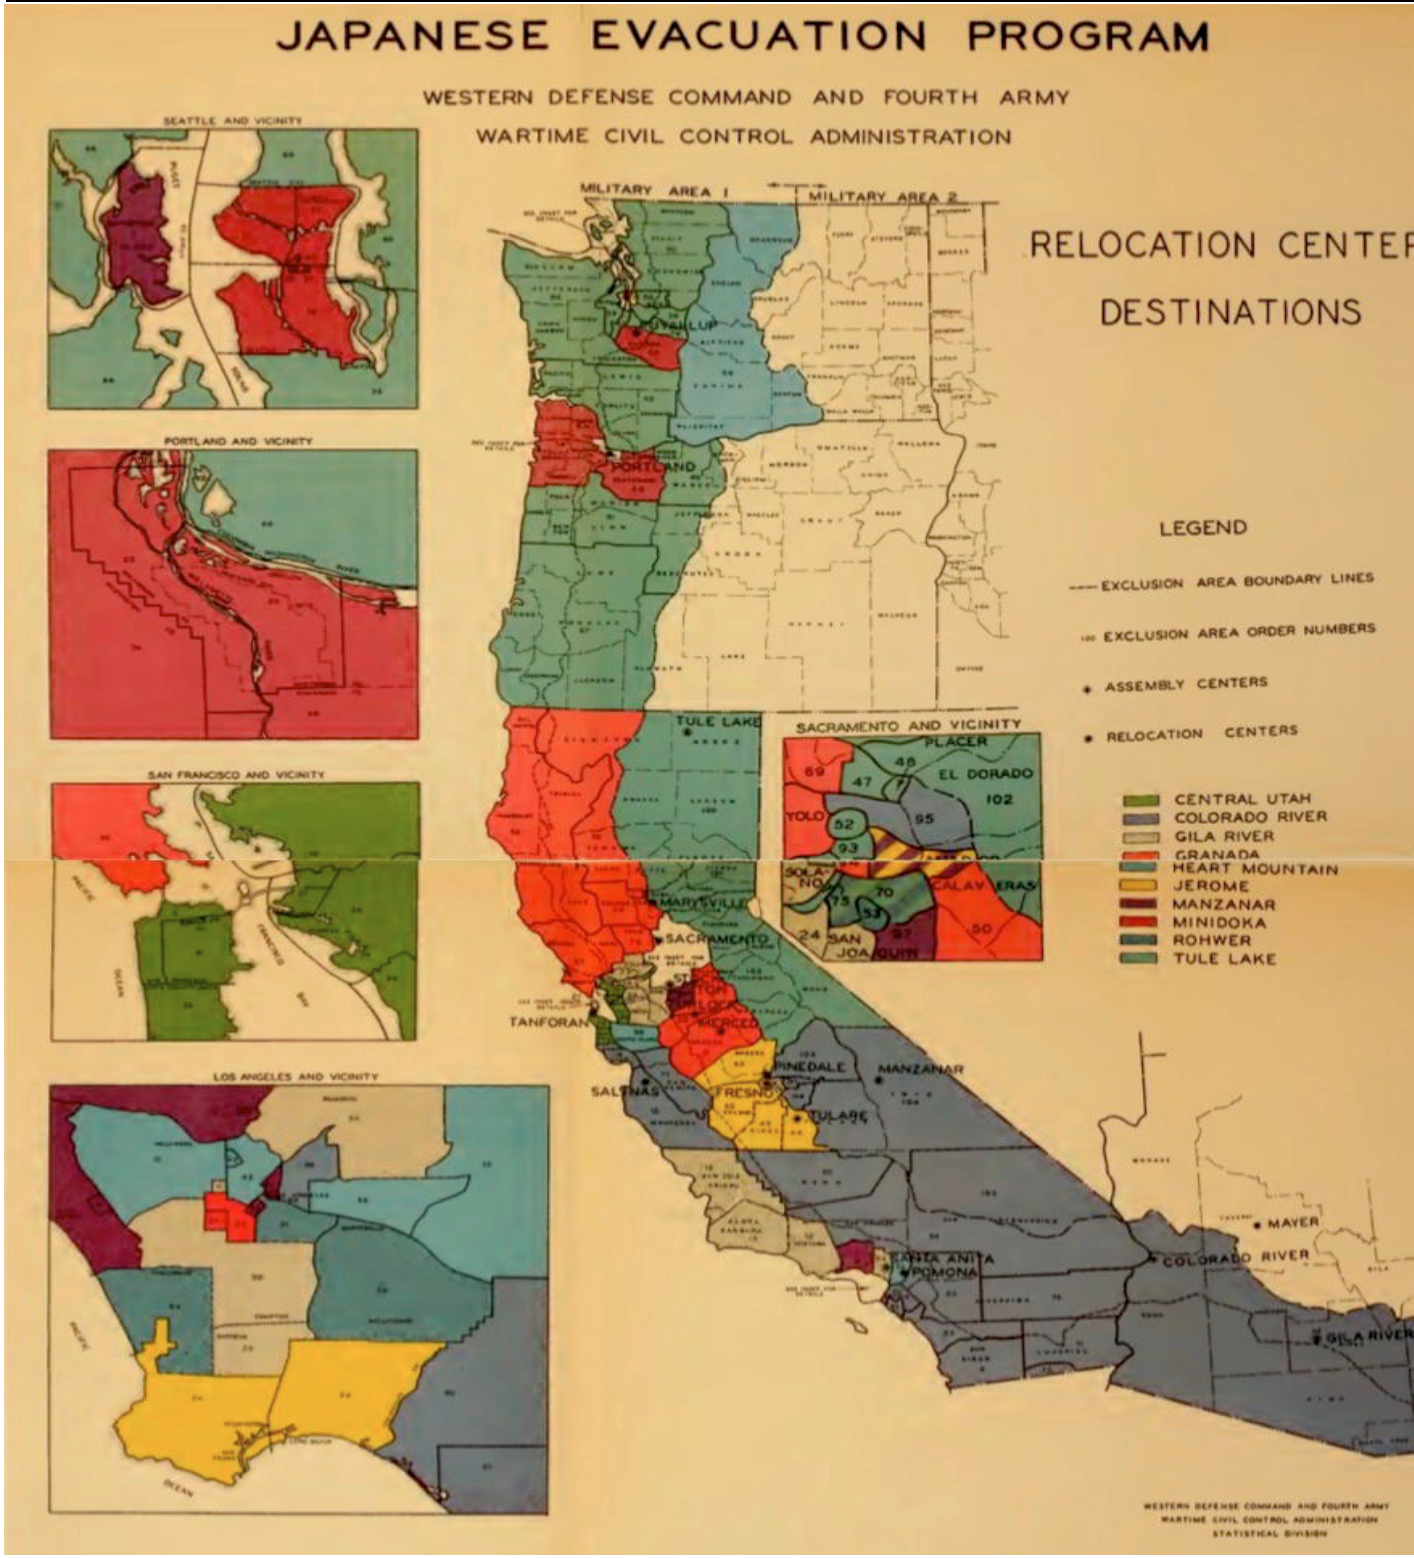
\includegraphics[height=5cm]{../figures/WRAzonesmap.png} \\
  \end{adjustbox}
  \footnotesize
    \emph{Note:}
  Interned proportions are calculated as the number of internees from the county
  divided by the county's Japanese population in the 1940 full-count census.
  Counties in white had zero Japanese respondents in the 1940 census.
  Color scale is restricted to show all counties with
  internment proportion of greater or equal to one as the same color.
  % The map on the below comes from the 1942 Western Defense Command's Final Report [cite/p:@dewittjohnl.FinalReportJapanese1943]
  % and shows in color the evacuation areas along the West Coast.
\end{figure}

The Exclusion Zone is clearly shown in this map
by the clustering of highly-interned counties in the southern half of Arizona,
California, and the western halfs of both Oregon and Washington.
However, based on the comparison between the 1940 census and the WRA records,
it seems that not all counties within the Exclusion Zone
were affected equally.
For example, in San Luis Obisbo County, California,
only 439 of the county's 932 Japanese residents in 1940
ended up in the camp lists.
There are also a few counties outside of the official Exclusion Zone
from which a few internees arrived
including Curry, New Mexico; Box Elder, Utah; and New York, New York.
This is likely due to either family reunification
or migration from those counties prior to 1942 to the West Coast.

Importantly for the later identifying assumptions in my empirical methods,
there is historical anecdotal evidence to suggest that these
voluntary migrants may have been an economically selected group.
Some Japanese living on the West Coast were permitted to leave the Exclusion Zone
if they had a sponsor living in another state who was able to prove that
they had a job or educational program in that state.
Some Japanese families were able to rely on business connections.
For example, in an interview with the
\href{https://ddr.densho.org/media/ddr-manz-1/ddr-manz-1-34-transcript-2e0e58d5a9.htm}{Densho Digital Archive},
Art Imagire recalls his mother's decision to move their family to Reno, Nevada
because one of her former clients offered her a job as a dress-maker there
\citep{imagireArtImagireInterview2008}.
Imagire cites his mother's value for her children's education
as an important reason for why their family was one of the few which chose,
``to drop everything and move''.
Additionally, several thousand Nisei were attending college
when Pearl Harbor was attacked.
Many Nisei students such as Sam Naito
were sent home from West Coast schools like the University of Oregon
during their academic term \citep{naitoSamNaitoInterview2003}.
Some, like Naito, were able to transfer to schools outside of the exclusion
zone to continue their education.

In my empirical strategy, I address this possibility that
some Japanese may have chosen to voluntarily migrate
by controlling for their observable 1940 characteristics
and by comparing against West Coast Chinese in the control group.

After two years of WRA camp operations, the government began to debate how to
end the evacuation orders towards the end of 1944. One statement issued on
December 9 illustrates that one of the initial goals of interment was actually
to cause a permanent shift in the Japanese American population away from the
West Coast as part of a wide-scale program of `deghettoization':
\begin{quote}
``One of the major WRA aims, from the beginning, has been to encourage the widest possible dispersal of evacuees throughout the Nation, and this will continue as a prime objective during the final phase of the program.''

-- \citet{commissiononwartimerelocationPersonalJusticeDenied1983}
\end{quote}

To the extent to which the relocation policies described above were successful,
this period of history provides an opportunity to examine
the way that contemporary or future displaced people
may potentially adapt to new labor markets and conditions.
\subsection{Motivating Literature}
\label{sec:orga90653c}

Several existing studies have tried to quantify the causal effect
of Japanese internment on long-term earnings
\citep{chinLongRunLaborMarket2005},
childhood health
\citep{saavedraEarlyChildhoodConditions2013,grossmanIntergenerationalHealthEffects2025},
and educational attainment
\citep{saavedraSchoolQualityEducational2015}.

On the other hand, other studies have identified surprising ways
in which internees did better than their counterparts.
\citep{shoagCausalEffectPlace2016} examine the persistent pattern of
internees' tendency to settle closer to their assigned camp,
and as a result find that differential exposure to more affluent areas
led to some internees experiencing more long-term upward mobility than others.
\citep{arellano-boverDisplacementDiversityMobility2022} finds that overall,
interned Japanese men experienced 9-22\% higher incomes
relative to similar Chinese and non-interned Japanese men.
He attributes this effect to a combination of information and skills transfers
among those living in camps together,
migration to new labor markets, and career switching
that would not have happened if internees had remained in their original homes
on the West Coast.

These economic findings are reinforced by more qualitative evidence
voiced by the Nisei themselves
and in historical research on this period.
\citep{taylorLeavingConcentrationCamps1991}
points to the differences in the benefits of relocation between
those who left earlier (1942-1944) via work or education programs,
and those who left in 1944 and 1945 who tended to be older
and more resistant to the government's policies.
\citep{austinEastwardPioneersJapanese2007}
highlights the experiences of several Nisei who resettled in cities such as
Chicago, Detroit and Minneapolis.
For those who faced discrimination on the West Coast
where anti-Japanese sentiment was more prevalent,
these new cities felt more socially welcoming
and economically promising.

Aside from the importance of understanding the losses to internees, Japanese
Internment can also serve as an interesting natural experiment through the
involuntary nature of the experiences of internees.
A key question in previous economic literature is the extent to which
geographic location influences economic outcomes, such as upward mobility or earnings.
It is difficult to provide an unbiased causal estimate because households usually
have a large degree of choice in where they live. Previous studies have used a
variety of empirical strategies to separate out this causal effect including
controlling for observable characteristics like education
\citep{glaeserCitiesSkills2001}, worker fixed-effects or
through leveraging other exogenous placements of households like the Moving to
Opportunity Experiment
\citep{chettyEffectsExposureBetter2016}.

Related to the overall racial discrimination faced by Japanese Americans,
Chinese Americans also faced immigration barriers
\citep{chenImpactSkillBasedImmigration2015},
and discrimination
\citep{chenInstitutionalDiscriminationAssimilation2024}.


Other research points to the importance of social networks for migration choices.
\citep{munshiSocialNetworksMigration2020}
expands the standard Roy model of migration choice
\citep{royThoughtsDistributionEarnings1951}
by adding the possibility for the number of individuals in a potential migrant's
social network living in a given destination to affect their utility
of living there themselves.
\section{Data}
\label{sec:org4e10131}
I combine historical data from two main sources
to track the economic outcomes of interned Japanese Americans
and compare them to similar groups who were not interned.
I first collect the demographic characteristics of internees
as they appear in the WRA camp records
together with geographic records on their county of origin before removal.
Then I combine statistics on the gemographic makeup of the WRA internee records
with overall demographics of Japanese Americans who appear in the 1940 full-count census
to construct an index of which counties and demographics among the Japanese population were more exposed to internment and removal.
I then apply this index of internment status to the set of Japanese and Chinese American census respondents who are linked across both the 1940 and 1950 censuses
to identify a sample of Japanese who are likely to be internees
and a comparison group from similar populations of Chinese non-West Coast Japanese linked respondents.
\subsection{WRA Records}
\label{sec:org3fee6d9}

The WRA kept detailed records of the process of relocating and incarcerating
the West Coast Japanese population.
I use the dataset from WRA Form 26: Evacuee Summary Data in the collection of
Records About Japanese Americans Interned During World War II
in the National Archives.
The original paper form from which this digitized version was coded
included each internee's name, previous address in 1942,
the assembly center and internment camp to which they were assigned,
their educational attainment, occupation,
and demographics including sex, birth year, and birthplace.

\begin{table}[!h]
\centering
\caption{Summary Statistics for WRA internees}
\label{tbl:wra_demog}
\begin{tabular}{lr}
\toprule\toprule
Dataset & Mean/Share \\
\midrule
\multicolumn{2}{l}{\textbf{WRA Data (N= 109,246)}} \\
\quad Male                                    & 0.55 \\
\quad Issei (1st generation)                  & 0.35 \\
\quad Mean (and st. dev.) age in 1942         & 30 (19) \\
\quad Mean (and st. dev.) immigration year    & 1916 (8) \\
\\
\multicolumn{2}{l}{\textbf{Top pre-war states}} \\
\quad California                              & 0.84 \\
\quad Washington                              & 0.12 \\
\quad Oregon                                  & 0.03 \\
\quad Hawaii                                  & 0.01 \\
\quad Arizona                                 & <0.01 \\
\quad Non West-Coast state                    & <0.01
\\
\multicolumn{2}{l}{\textbf{Top occupations}} \\
\quad Not employed/missing                    & 0.48 \\
\quad Farm hands, vegetables                  & 0.05 \\
\quad Farm hands, fruit                       & 0.04 \\
\quad Truck farmers                           & 0.04 \\
\quad Sales clerks                            & 0.04 \\
\quad Retail managers                         & 0.03 \\
\quad Gardeners and groundskeepers            & 0.02 \\
\quad Maids, general                          & 0.02 \\
\quad Farm managers and foremen               & 0.02 \\
\quad other                                   & 0.34 \\
\bottomrule
\end{tabular}

{\footnotesize\emph{Note:}

\emph{Source:} Japanese-American Internee Data File, 1942 - 1946, National Archives
}
\end{table}


Table \ref{tbl:wra_demog} reports a summary of the main demographic variables
of internees compared to the full 1940 Japanese population.
Internees represented a large majority (86\%)
of the Japanese population in the U.S. in 1940.
Internees were representative of the population in terms of their education,
gender composition, and country of birth.
The 65\% of internees born in the U.S.
represent the generation known as the ``Nisei'',
or second generation after their parents,
the ``Issei'', who make up most of the remaining 35\% of internees.
The average Issei was born in 1890,
and would have been in their early fifties during internment,
while the average Nisei was born in 1927
and would have been a teenager when interned.

Figure \ref{fig:internee-ages} shows the distribution
of the age of internees at the time of the evacuation order in 1942.
This figure reveals that there was a large variation in the ages of internees
and that the ten camps were fairly balanced in their age composition.
The most prominent age range in this figure is made up of young adults
between the ages of 15 and 25.

The WRA records also provide a mapping from the county of residence of all internees to the first camp they were placed.
Table \ref{tbl:cmp-cty} groups all internees by their previous address and their assigned camp.
The 20 largest counties with more than 1,000 interned residents are shown broken down by each of the ten camps.

Among the main internment counties are the major West Coast urban areas of Los Angeles, Seattle, Sacramento, San Francisco, and Portland.
However, there is also a large number of internees from more rural counties in California including Fresno, San Joaquin, Placer, and Tulare.
Interned Japanese came from a variety of backgrounds shown here by the range of urban and rural counties,
and also reflected in the range of occupations held by internees.

The WRA records give a
(nearly\footnote{Some internees were sent to prisons operated by the Department of Justice which were not included in the WRA records.})
complete list of all individuals who were interned during World War II.
In the next section, I use the demographics of this group of documented internees
to estimate the likelihood of internment for individuals who appear in separate census records.
\subsection{Comparison Groups by Estimated Internment Status}
\label{sec:org5c2202d}

My main analysis compares Japanese individuals who are likely to have been interned
against other Japanese and Chinese individuals who were most likely not interned.
Because the census does not ask about a person's actual internment status,
I apply a non-parametric estimator from \citep{arellano-boverDisplacementDiversityMobility2022} to infer an individual's actual internment status using their demographic characteristics and original place of residence before the war.

My goal with bringing the MLP linked census data
together with the WRA internment camp data
is to create an individual-level panel data set
which includes both those persons who are likely internees
and a control group of people who were almost certainly not interned
(and considered untreated in the natural experiment of internment).
In a hypothetical experiment with the goal of identifying the causal effect
of forced relocation and incarceration on individual earnings,
a random set of workers could have been selected from the West Coast
and sent to random destinations in the rest of the US.
In that case, a simple comparison of earnings in the displaced group
against the earnings of the workers on the West Coast who were not interned
would return the causal effect of interest.
Although in some ways Japanese internment does resemble a natural experiment,
there are some important ways in which internment differed from this hypothetical,
which I will address in this section to motivate the main empirical strategy.

Precisely because internment was specifically targeted based on Japanese ancestry,
assignment to treatment was non-random.\footnote{There were several thousand Americans of German and Italian ancestry who were also interned during this period, although the overall magnitude was less than the group of Japanese internees and much less as a proportion of the existing German and Italian immigrant populations.}

If we simply compare interned Japanese earnings after the war
to all other residents of the West Coast,
then our estimate of internment's effect
will be biased downward if Japanese were already restricted from
joining certain occupations by discrimination.
One potential comparison group for  West Coast Japanese is Hawaiian Japanese,
a large population that was not subject to internment
for economic reasons \citep{chinLongRunLaborMarket2005}.
However, we could expect that Japanese Hawaiians
would have experienced higher growth in their earnings
compared to their West Coast peers even without the effect of internment.
The Japanese population in Hawaii was more economically integrated
in especially nonagricultural occupations
and could have experienced less of the postwar anti-Japanese discrimintation.

Another potential comparison group is Japanese living in mainland states
that were not subject to internment.
However, because such a large proportion of the mainland Japanese population
was living in Arizona, California, Oregon, or Washington
(about 90\% in the 1940 full-count census data),
this leaves a smaller control group.
Additionally, those Japanese immigrants who had already moved east away
from the point of entry on the West Coast
were likely to already be self-selected individuals
who would have had more access to higher-earning job opportunities
due to education or skills.

For the reasons above,
I follow \citet{arellano-boverDisplacementDiversityMobility2022}
by including Chinese Americans in my main sample
together with all mainland Japanese.
Chinese immigrants entered the US West Coast
around the same time as the major wave of Japanese immigration.
Japanese workers were also seen as a substitute for cheap Chinese labor
for work on the transcontinental railroads and in agriculture
\citep{chenImpactSkillBasedImmigration2015}.
Chinese Americans were not included in any of the relocation
or internment orders following Executive Order 9066,
but in the absence of internment,
their wages and employment would likely have continued to evolve similarly
to those of the West Coast Japanese population.
For these reasons, Chinese Americans make a natural comparison group
to recreate the counterfactual earnings outcomes interned Japanese
would have had if they had never been interned.
\subsubsection{Voluntary Migration}
\label{sec:orgb77fa42}
Although all persons of Japanese descent living on the West Coast
were ordered to evacuate outside of the Exclusion Zone
(and no Chinese persons were ordered to evacuate),
the ability of some Japanese to self-evacuate
means some were able to avoid being sent to any of the ten internment camps.
\citet{dewittjohnl.FinalReportJapanese1943} puts the number of
voluntary evacuees at 4,889.
A research design that treats all Japanese living on the West Coast in 1940
as the treatment group ignores this number
as well as any voluntary emigration by Japanese
from the West Coast to other states.
In order to obtain a more accurate estimate of the actual
probability that any individual Japanese census respondent was a true internee,
I create a measure of predicted internee status
which compares the number of internees in the WRA camp records
against the number of Japanese living in each county in the 1940 census.

The discrepancy between 1940 Japanese residents and internee origins
could be due to several reasons.
General demographic changes such as births and deaths
could mean that not everyone who responded to the census was still alive in 1942,
or that some children who appear in the internment camps
had yet to be born in 1940.
Voluntary migration could also affect these interment proportions.
Some may have migrated between counties before Pearl Harbor,
or even chosen to move outside the Exclusion Zone
during the period when voluntary migration was encouraged by the Army.
If inter-county migration within the West Coast was widespread during this period,
that could mean that some West Coast Japanese who are identified as internees
based on their 1940 county
were actually able to escape the WRA camps.
In this case, it might be more appropriate to interpret the effect of
the predicited internment status estimated here
as the effect of evacuation orders for Japanese overall,
including migration by those who were not actually interned.

Some counties have a proportion greater than one when calculated this way.
For example, one of the thirty counties affected by this is
Sacramento County in California,
which had a Japanese population of 6,851 in the 1940 census
but in the WRA records there are 7,827 internees who are reported
as coming from Sacramento County.
Although I use this proportion as a measure of internment status
for the linked individuals from each affected county,
it is important to note that this internment status is not a true probability.

The method of using county-level internment proportions
as a proxy for an individual Japanese worker's own internment status
makes the identifying assumption that
Japanese within the same county had equal chances of being interned.
This would be violated if some types of workers were able to avoid internment
for reasons endogenous to their labor market outcomes.
As I discuss in section \ref{sec:orge28ed0c},
voluntary evacuees did anecdotally seem to be more likely to relocate
for educational reasons,
or because of family and social networks living in the East.
If the types of Japanese who were more likely to be able to voluntarily evacuate
were also more likely to earn higher wages,
then the estimated effect of internment on postwar earnings will
be biased upward.

To account for this possibility,
I also include an internment status for the linked MLP sample
using the method described in
\citet{arellano-boverDisplacementDiversityMobility2022}
which conditions on additional demographic variables.
Following his application of Bayes' Rule,
the probability that an individual \(i\)
in the demographic group \(z\) who lived in county \(c\) in 1942 was interned
(\(Pr(I_{i}=1|z_i,c(i))\))
could be determined from the proportion of the whole population who were interned
(\(Pr(I_{i}=1)\),
the proportion of the population with demographics \(z\)
who lived in county \(c\) in 1942, \(Pr(c(i)_{42}, z_i)\),
and the probability of a known internee
having the same demographics and county in 1942,
\(Pr(c(i)_{42}, z_i|I_i=1)\):

$$
Pr(I_i=1|z_i, c(i)_{42}) =
\frac{Pr\left(c(i)_{42}, z_i|I_i=1\right) \cdot Pr(I_i=1)}{Pr(c(i)_{42}, z_i)}.
$$

However, because my target sample of census respondents
was only asked about their county of residence in the year of the census
and not in 1942, \(c(i)_{40}\) is used as a proxy
for census respondents' 1942 locations.

The estimator for the true internment status of a census respondent is:

\begin{equation}\label{eq:predint}
\hat{E}[I|c(i), z_i] =
\frac{n(j |c(i)_{40}=c(j)_{42} , ~ z_i=z_j)_{j\in \{j | I_j = 1\}}}
{n(k | c(i)_{40}=c(k)_{40}, ~ z_i=z_k)_{k\in K}}.
\end{equation}

The numerator represents the number of individuals \(j\)
who match linked individual \(i\) on origin county and demographics
in the WRA internment records (so that \(I_j = 1\) for certain).
The denominator represents the number of individuals \(k\) from the 1940 census
who match \(i\)'s county and demographics.

This will produce a biased estimate of true internment status
if there were unobserved changes in population
in each county between 1940 and 1942.
For example, for a county that experienced a net outflow of residents,
then the ratio of residents in 1940 to 1942 would be greater than 1
and we would have an estimated internment probability
that overstates the likelihood that a resident of county \(c\) in 1940
would be interned.

\begin{table}[!h]
\centering
\caption{\label{tab:tbl:intern_groups}Internment Status by Demographic Group}
\centering
\begin{threeparttable}
\begin{adjustbox}{width=\textwidth, center}
\begin{tabular}[t]{rlllrr}
\toprule
Rank & Sex & Birthplace & Birth year & \shortstack{Observations\\(1940 Census)} & \shortstack{Internment\\index}\\
\midrule
\addlinespace[0.3em]
\multicolumn{6}{l}{\textbf{Most interned}}\\
\hspace{1em}1 & Male & Japan & 1870-1879 & 4271 & 1.03\\
\hspace{1em}2 & Female & Japan & 1880-1889 & 2918 & 1.01\\
\hspace{1em}3 & Female & West Coast (AZ, CA, OR, WA) & 1910-1919 & 7504 & 1.01\\
\hspace{1em}4 & Male & Alaska, Hawaii, other & 1920-1929 & 136 & 1.00\\
\hspace{1em}5 & Male & Alaska, Hawaii, other & 1900-1909 & 830 & 1.00\\
\hspace{1em}6 & Female & Japan & 1890-1899 & 7052 & 0.97\\
\hspace{1em}7 & Female & Japan & 1870-1879 & 830 & 0.95\\
\hspace{1em}8 & Male & Japan & 1880-1889 & 9928 & 0.95\\
\hspace{1em}9 & Female & West Coast (AZ, CA, OR, WA) & 1900-1909 & 781 & 0.94\\
\hspace{1em}10 & Male & Japan & 1860-1869 & 443 & 0.93\\
\addlinespace[0.3em]
\multicolumn{6}{l}{\textbf{Medium internment}}\\
\hspace{1em}27 & Female & Japan & 1860-1869 & 95 & 0.53\\
\hspace{1em}28 & Male & Japan & 1920-1929 & 210 & 0.51\\
\hspace{1em}29 & Male & Rest of Continental US & 1920-1929 & 565 & 0.45\\
\hspace{1em}30 & Female & Rest of Continental US & 1920-1929 & 473 & 0.44\\
\hspace{1em}31 & Female & Japan & 1910-1919 & 512 & 0.44\\
\hspace{1em}32 & Female & Rest of Continental US & 1910-1919 & 385 & 0.43\\
\hspace{1em}33 & Male & Japan & NA & 22 & 0.41\\
\hspace{1em}34 & Male & Japan & 1910-1919 & 666 & 0.41\\
\hspace{1em}35 & Female & Japan & 1930-1939 & 69 & 0.41\\
\addlinespace[0.3em]
\multicolumn{6}{l}{\textbf{Least interned}}\\
\hspace{1em}41 & Female & Rest of Continental US & 1930-1939 & 96 & 0.24\\
\hspace{1em}42 & Female & West Coast (AZ, CA, OR, WA) & 1890-1899 & 68 & 0.22\\
\hspace{1em}43 & Female & Alaska, Hawaii, other & 1880-1889 & 10 & 0.20\\
\hspace{1em}44 & Male & West Coast (AZ, CA, OR, WA) & 1890-1899 & 104 & 0.19\\
\hspace{1em}45 & Female & Rest of Continental US & 1900-1909 & 32 & 0.19\\
\hspace{1em}46 & Female & Japan & NA & 14 & 0.14\\
\hspace{1em}47 & Male & Rest of Continental US & 1930-1939 & 107 & 0.14\\
\hspace{1em}48 & Male & Rest of Continental US & 1900-1909 & 36 & 0.08\\
\hspace{1em}49 & Female & West Coast (AZ, CA, OR, WA) & 1880-1889 & 19 & 0.05\\
\hspace{1em}50 & Male & West Coast (AZ, CA, OR, WA) & 1880-1889 & 52 & 0.02\\
\bottomrule
\end{tabular}
\end{adjustbox}
\begin{tablenotes}
\item Proportions of interned Japanese in the WRA records out of the number of individuals in the 1940 full-count census in each demographic group.
\end{tablenotes}
\end{threeparttable}
\end{table}
\subsection{Linked Census Microdata}
\label{sec:orga466988}

I collect economic and demographic data on the populations of interest
from the full count decennial censuses taken in 1940 and 1950
\citep{rugglesIPUMSAncestryFull2024}.
IPUMS also provides linked individual census data up until 1950
through their Multigenerational Longitudinal Panel (MLP) project
\citep{rugglesIPUMSMultigenerationalLongitudinal2025}.
I use the links between the 1940 and 1950 full-count censuses
from version 2.0 of the MLP data provided by IPUMS.

For my main analysis sample,
I select all individuals
whose reported race in 1940 was either Japanese or Chinese,
who born before 1926 (so that they would have been of working age by World War II),
and who are not missing income or employment data in either census.
This leaves me with a linked sample of 8,136 individuals,
of which about three quarters of whom are Japanese
and one quarter are Chinese.

\begin{table}
  \caption{\label{tbl:mlp_sumstats}Summary statistics for Chinese and Japanese linked in MLP}
  \begin{adjustbox}{width=.9\textwidth, center}
\begin{tblr}[         %% tabularray outer open
]                     %% tabularray outer close
{                     %% tabularray inner open
colspec={Q[]Q[]Q[]Q[]Q[]Q[]Q[]},
cell{2}{1}={}{halign=l,},
cell{3}{1}={}{halign=l,},
cell{4}{1}={}{halign=l,},
cell{5}{1}={}{halign=l,},
cell{6}{1}={}{halign=l,},
cell{7}{1}={}{halign=l,},
cell{8}{1}={}{halign=l,},
cell{9}{1}={}{halign=l,},
cell{10}{1}={}{halign=l,},
cell{11}{1}={}{halign=l,},
cell{12}{1}={}{halign=l,},
cell{13}{1}={}{halign=l,},
cell{14}{1}={}{halign=l,},
cell{15}{1}={}{halign=l,},
cell{16}{1}={}{halign=l,},
cell{17}{1}={}{halign=l,},
cell{18}{1}={}{halign=l,},
cell{19}{1}={}{halign=l,},
cell{1}{1}={}{halign=l, halign=c,},
cell{2}{2}={}{halign=r,},
cell{2}{3}={}{halign=r,},
cell{2}{4}={}{halign=r,},
cell{2}{5}={}{halign=r,},
cell{2}{6}={}{halign=r,},
cell{2}{7}={}{halign=r,},
cell{3}{2}={}{halign=r,},
cell{3}{3}={}{halign=r,},
cell{3}{4}={}{halign=r,},
cell{3}{5}={}{halign=r,},
cell{3}{6}={}{halign=r,},
cell{3}{7}={}{halign=r,},
cell{4}{2}={}{halign=r,},
cell{4}{3}={}{halign=r,},
cell{4}{4}={}{halign=r,},
cell{4}{5}={}{halign=r,},
cell{4}{6}={}{halign=r,},
cell{4}{7}={}{halign=r,},
cell{5}{2}={}{halign=r,},
cell{5}{3}={}{halign=r,},
cell{5}{4}={}{halign=r,},
cell{5}{5}={}{halign=r,},
cell{5}{6}={}{halign=r,},
cell{5}{7}={}{halign=r,},
cell{6}{2}={}{halign=r,},
cell{6}{3}={}{halign=r,},
cell{6}{4}={}{halign=r,},
cell{6}{5}={}{halign=r,},
cell{6}{6}={}{halign=r,},
cell{6}{7}={}{halign=r,},
cell{7}{2}={}{halign=r,},
cell{7}{3}={}{halign=r,},
cell{7}{4}={}{halign=r,},
cell{7}{5}={}{halign=r,},
cell{7}{6}={}{halign=r,},
cell{7}{7}={}{halign=r,},
cell{8}{2}={}{halign=r,},
cell{8}{3}={}{halign=r,},
cell{8}{4}={}{halign=r,},
cell{8}{5}={}{halign=r,},
cell{8}{6}={}{halign=r,},
cell{8}{7}={}{halign=r,},
cell{9}{2}={}{halign=r,},
cell{9}{3}={}{halign=r,},
cell{9}{4}={}{halign=r,},
cell{9}{5}={}{halign=r,},
cell{9}{6}={}{halign=r,},
cell{9}{7}={}{halign=r,},
cell{10}{2}={}{halign=r,},
cell{10}{3}={}{halign=r,},
cell{10}{4}={}{halign=r,},
cell{10}{5}={}{halign=r,},
cell{10}{6}={}{halign=r,},
cell{10}{7}={}{halign=r,},
cell{11}{2}={}{halign=r,},
cell{11}{3}={}{halign=r,},
cell{11}{4}={}{halign=r,},
cell{11}{5}={}{halign=r,},
cell{11}{6}={}{halign=r,},
cell{11}{7}={}{halign=r,},
cell{12}{2}={}{halign=r,},
cell{12}{3}={}{halign=r,},
cell{12}{4}={}{halign=r,},
cell{12}{5}={}{halign=r,},
cell{12}{6}={}{halign=r,},
cell{12}{7}={}{halign=r,},
cell{13}{2}={}{halign=r,},
cell{13}{3}={}{halign=r,},
cell{13}{4}={}{halign=r,},
cell{13}{5}={}{halign=r,},
cell{13}{6}={}{halign=r,},
cell{13}{7}={}{halign=r,},
cell{14}{2}={}{halign=r,},
cell{14}{3}={}{halign=r,},
cell{14}{4}={}{halign=r,},
cell{14}{5}={}{halign=r,},
cell{14}{6}={}{halign=r,},
cell{14}{7}={}{halign=r,},
cell{15}{2}={}{halign=r,},
cell{15}{3}={}{halign=r,},
cell{15}{4}={}{halign=r,},
cell{15}{5}={}{halign=r,},
cell{15}{6}={}{halign=r,},
cell{15}{7}={}{halign=r,},
cell{16}{2}={}{halign=r,},
cell{16}{3}={}{halign=r,},
cell{16}{4}={}{halign=r,},
cell{16}{5}={}{halign=r,},
cell{16}{6}={}{halign=r,},
cell{16}{7}={}{halign=r,},
cell{17}{2}={}{halign=r,},
cell{17}{3}={}{halign=r,},
cell{17}{4}={}{halign=r,},
cell{17}{5}={}{halign=r,},
cell{17}{6}={}{halign=r,},
cell{17}{7}={}{halign=r,},
cell{18}{2}={}{halign=r,},
cell{18}{3}={}{halign=r,},
cell{18}{4}={}{halign=r,},
cell{18}{5}={}{halign=r,},
cell{18}{6}={}{halign=r,},
cell{18}{7}={}{halign=r,},
cell{19}{2}={}{halign=r,},
cell{19}{3}={}{halign=r,},
cell{19}{4}={}{halign=r,},
cell{19}{5}={}{halign=r,},
cell{19}{6}={}{halign=r,},
cell{19}{7}={}{halign=r,},
cell{1}{3}={}{halign=r, halign=c,},
cell{1}{5}={}{halign=r, halign=c,},
cell{1}{6}={}{halign=r, halign=c,},
cell{1}{7}={}{halign=r, halign=c,},
cell{1}{2}={c=2,}{halign=r, halign=c, halign=c,},
cell{1}{4}={c=2,}{halign=r, halign=c, halign=c,},
}                     %% tabularray inner close
\toprule
& Chinese (N=2069) &  & Japanese (N=6067) &  &  &  \\ \cmidrule[lr]{2-3}\cmidrule[lr]{4-5}
& Mean & Std. Dev. & Mean & Std. Dev. & Diff. in Means & Std. Error \\ \midrule %% TinyTableHeader
Year of birth & \num{1904.3} & \num{12.7} & \num{1904.0} & \num{14.9} & \num{-0.3} & \num{0.3} \\
Female & \num{0.3} & \num{0.4} & \num{0.4} & \num{0.5} & \num{0.2} & \num{0.0} \\
Farm status 1940 & \num{0.0} & \num{0.2} & \num{0.4} & \num{0.5} & \num{0.4} & \num{0.0} \\
Farm status 1950 & \num{0.0} & \num{0.1} & \num{0.2} & \num{0.4} & \num{0.2} & \num{0.0} \\
Wage income 1939 & \num{625.2} & \num{1027.5} & \num{407.5} & \num{845.2} & \num{-217.8} & \num{25.1} \\
Wage income 1949 & \num{1151.1} & \num{1578.1} & \num{1004.2} & \num{1452.0} & \num{-146.9} & \num{39.4} \\
Business/farm income 1949 & \num{580.6} & \num{1355.8} & \num{567.7} & \num{1330.1} & \num{-12.9} & \num{34.5} \\
Other income 1949 & \num{275.1} & \num{989.3} & \num{256.8} & \num{951.9} & \num{-18.4} & \num{25.1} \\
OCCSCORE 1940 & \num{15.4} & \num{15.1} & \num{11.4} & \num{13.1} & \num{-4.0} & \num{0.4} \\
OCCSCORE in 1950 & \num{17.6} & \num{16.7} & \num{12.7} & \num{13.1} & \num{-4.8} & \num{0.4} \\
Weeks worked in 1939 & \num{27.8} & \num{24.0} & \num{26.7} & \num{24.2} & \num{-1.1} & \num{0.6} \\
Weeks worked in 1949 & \num{30.5} & \num{23.1} & \num{30.6} & \num{22.4} & \num{0.1} & \num{0.6} \\
Hours worked last week (1940) & \num{28.1} & \num{27.5} & \num{26.4} & \num{27.0} & \num{-1.7} & \num{0.7} \\
Hours worked last week (1950) & \num{29.0} & \num{25.9} & \num{28.0} & \num{25.4} & \num{-1.0} & \num{0.7} \\
% Was employed 1940 & \num{1.6} & \num{0.5} & \num{1.6} & \num{0.5} & \num{-0.0} & \num{0.0} \\
% Was employed 1950 & \num{1.7} & \num{0.5} & \num{1.6} & \num{0.5} & \num{-0.0} & \num{0.0} \\
% Moved counties 1940-1950 & \num{1.2} & \num{0.4} & \num{1.4} & \num{0.5} & \num{0.2} & \num{0.0} \\
\bottomrule
\end{tblr}

\end{adjustbox}
{\tiny \emph{Note:} Observations include all individuals linked by \href{https://usa.ipums.org/usa/mlp/mlp.shtml}{MLP} whose reported race is either Chinese or Japanese in 1940 and who have non-missing income data in both the 1940 and 1950 census.}
\end{table}

Table \ref{tbl:mlp_sumstats} reports summary statistics for this sample,
broken down by race.
Japanese and Chinese are similar in age,
with both groups having an average year of birth of 1904.
Within the Chinese population, men are overrepresented,
with 72\% being male compared to 58\% male in the Japanese population.
The 1940 census only asked about income earned through wages and employment
in the previous year.
However, the 1950 census added questions about other forms of income
including income from respondents who owned their own businesses or farms.
OCCSCORE is a variable provided by IPUMS
which ranks the occupations of census respondents
by the median wage that was earned for persons with the same occupation.
Both censuses asked about the number of weeks each person reported working
in the previous year,
as well as the number of hours they worked in the previous week.
Employment status for this working-age sample
is equal to one if the person reported being employed,
and equal to zero if they were unemployed or not in the labor force.
I categorize unemployed persons
together with those who are not in the labor force
to acknowledge the fact that internees may have been discouraged from
participating in the formal labor force due to trauma or discrimination.
\% insert citations here to back up this story.
Farm status in either year depends on whether the respondent's family
lived on a farm or not.
I take the county of residence reported by each linked respondent
and categorize each as a  migrant over this period
if the county they report in 1940 is different from their county in 1950.

In terms of economic characteristics,
the Japanese sample started with lower wages, fewer weeks and hours worked,
lower employment rates,
and lower-ranked occupations in the 1940 census compared to the Chinese sample.
However, the gap in wage income seems to have decreased by 1950.
In section \ref{sec:org33d384e}, I show evidence that
internment itself may have caused the Japanese population to earn higher wages
over this period than they would have otherwise earned.
The gap in weeks worked also seems to close between these two populations,
although the differences in hours worked and occupation score
do not seem to change between 1940 and 1950.

\label{Migration-differences}
Migration rates for Japanese are much higher than for Chinese over this period
(35\% vs 17\%).
Most of this is likely because the majority of the Japanese population
were interned and forcibly removed from their original 1940 counties.
However, some may be due to voluntary migration
before internment orders went into effect
or after their release from the WRA camps.

In order to determine internment status at a more granular level,
I use the distribution of internees' original counties of residence
from the 1940s camp records,
which I describe in the following section.

\begin{figure}
  \caption{Income distributions by treatment group and census year} \centering
  \label{fig:group-incwage-dist}
  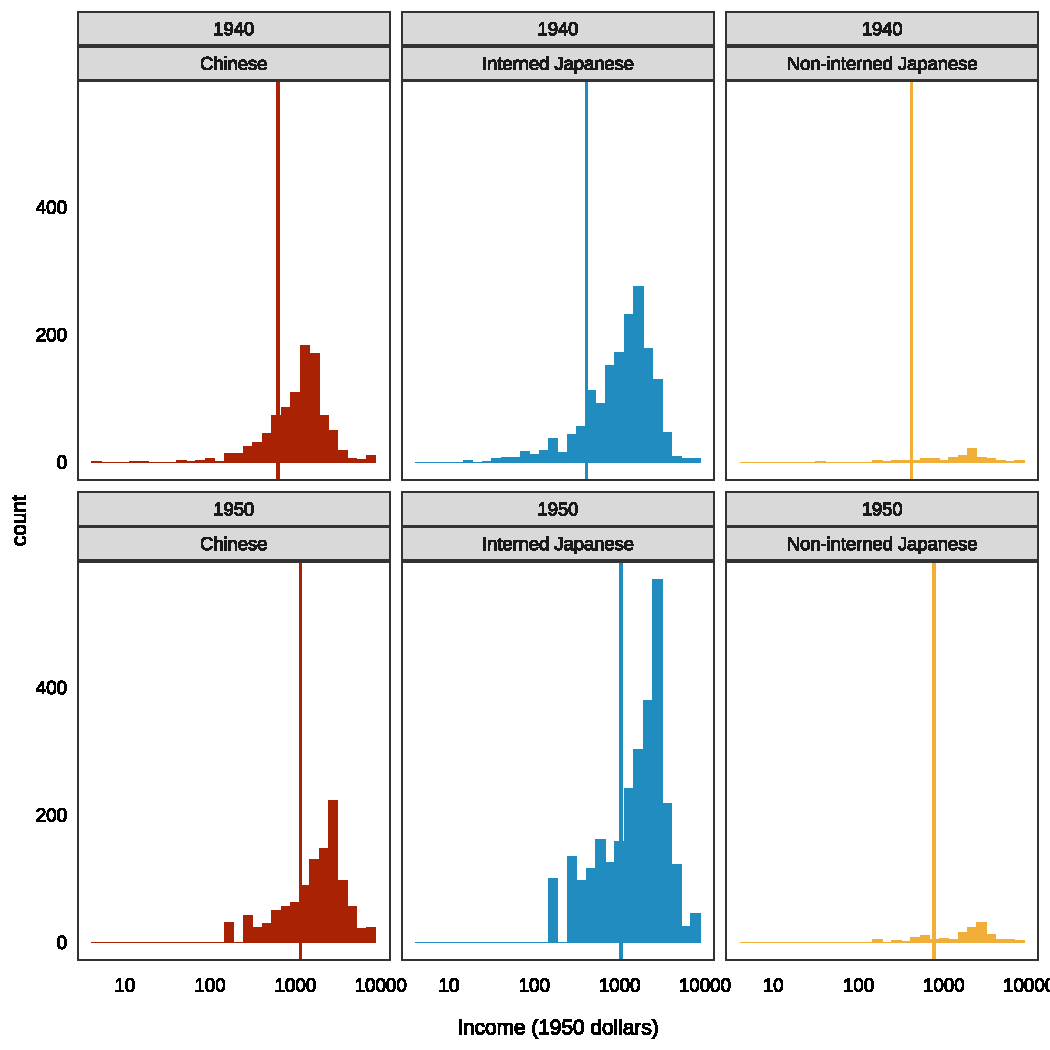
\includegraphics[width=\textwidth]{../figures/group-incwage-dist.pdf} \\
  \caption*{
    \footnotesize
    \emph{Note:}
    The top row is the distributions of income in 1940,
    the bottom row is distributions of 1950 income.
    All Chinese individuals are treated as non-interned.
    `Interned Japanese' include all Japanese individuals
    with an estimated probability of greater than 0.75.
    `Non-interned Japanese' include all Japanese
    with an estimated probability equal to zero.
    Japanese with a probability between 0 and 0.75 are omitted
    in this figure.
    Income is the total earnings through wage employment
    from the year prior to each census year.
    Incomes in 1940 are adjusted for inflation to 1950 dollar amounts.
    Vertical lines represent the group averages.
    }
\end{figure}

Figure \ref{fig:group-incwage-dist} shows the histograms of
the natural log of INCWAGE,
the total earnings from wages and employment
(as opposed to earnings from self-employment, farming, etc.),
across the three different treatment groups\footnote{see section \ref{eq:predint} for more details}
among the linked MLP sample.
The first column shows that Chinese in the control group did experience
real wage growth on average over these ten years.
The difference in the Chinese log income distribution shown here
translates into an average increase in wages of 84\%
(an increase from \$625 in 1940 to \$1151 in 1950).
Although interned Japanese and non-interned Japanese
both started with similarly low wages compared to the Chinese sample
(\$411 and \$419, respectively),
by 1950, the Japanese who were likely interned almost closed the gap
in average income compared to the Chinese (\$1037 vs \$1151),
while the non-interned Japanese still lagged behind
with an average wage of \$769.

In section \ref{sec:methods}, I describe the methodological tools I use
to argue that the convergence I observe between the likely internee group
and their outperformance relative their non-interned peers
captures a causal effect of internment and forced relocation
on the incomes earned in 1950.
\section{Effects of Internment}
\label{sec:orgf1ec2d8}
\subsection{Descriptive Statistics for Internees and Comparison Groups}
\label{sec:orgb5b1d7e}
\subsection{Effect of Internment on Earnings}
\label{sec:org0999d97}
\subsubsection{Estimation Strategy}
\label{sec:orgf16b137}
To measure the effect of internment on earnings,
my main analysis uses the following specification:

\begin{equation}\label{eq:mainreg}
  Y_i = \alpha + \beta \hat{E}[I|c(i), z_i] + \mathbb{X}_i \Gamma + \epsilon_i
\end{equation}.

The main outcome of interest which I use for \(Y_i\)
is the reported dollar earnings of individual \(i\) in the 1950 census.
\(\alpha\) is an intercept term common to all linked individuals.
The vector of individual-level controls in \(\mathbb{X}\)
includes age, sex, and individual \(i\)'s earnings from the 1940 census,
adjusted to 1950 dollars.
In some specifications,
I also apply a fixed effect for the state
in which individual \(i\) was living in 1950

The probability of individual \(i\) being an internee, \(Pr(I)_i\),
is replaced by my estimated version from equation \ref{eq:predint}
using individual \(i\)'s reported race in 1940 as the only demographic \(z\).
The main causal effect of interest is represented by the estimator \(\beta\),
which represents the number of dollars of income
which an individual is estimated to have gained (or lost)
when moving from a non-internee to a likely internee.

A traditional difference-in-differences approach would require the
identifying assumption that both treated and untreated groups
would experience parallel trends in earnings in the absence of internment.
However, if individuals who had pre-existing advantages in the labor market
were able to self-select out of internment through voluntary migration,
then this parallel trends assumption would be violated.
By directly controlling for pre-internment income for each linked individual,
I address this concern for the variables that I do observe consistently
across censuses.

While this empirical strategy does not control
for all time-invariant unobservable factors,
the historical evidence suggests that
observables such as geographic location, education, and pre-war earnings
were the primary factors that determined the ways in which
internment and evacuation policies were individually enforced.
\subsubsection{Results}
\label{sec:orgd71b4da}
In this section I report the outcomes from the main linked sample
described in section \ref{sec:orga466988}
and estimated coefficients from section \ref{sec:wage-reg}.

\begin{table}[htbp]
   \caption{\label{tbl:reg1} Earning effects of internment}
   \bigskip
   \centering
   \begin{tabular}{lcccc}
      \toprule
       & \multicolumn{4}{c}{Income in 1950}\\
                                   & (1)     & (2)             & (3)             & (4)\\  
      \midrule 
      Internment Status            & -42.07  & 232.4$^{***}$   & 250.7$^{***}$   & 80.90\\   
                                   & (36.02) & (60.49)         & (59.86)         & (91.11)\\   
      Age                          &         & 33.30$^{***}$   & 12.45           & 11.22$^{**}$\\   
                                   &         & (7.837)         & (8.210)         & (4.786)\\   
      Age square                   &         & -0.5353$^{***}$ & -0.3143$^{***}$ & -0.3024$^{***}$\\   
                                   &         & (0.0808)        & (0.0835)        & (0.0461)\\   
      Male                         &         & 645.4$^{***}$   & 487.5$^{***}$   & 488.3$^{***}$\\   
                                   &         & (33.47)         & (35.14)         & (17.22)\\   
      Japanese                     &         & -210.0$^{***}$  & -246.2$^{***}$  & -98.45\\   
                                   &         & (63.93)         & (64.55)         & (88.69)\\   
      Income in 1940               &         &                 & 0.2409$^{***}$  & 0.2334$^{***}$\\   
                                   &         &                 & (0.0189)        & (0.0218)\\   
       \\
      Standard-Errors & \multicolumn{3}{c}{IID} & State$_{1940}$ \\ 
      Observations                 & 8,136   & 8,136           & 8,136           & 8,136\\  
      R$^2$                        & 0.00017 & 0.07616         & 0.10227         & 0.10882\\  
      Within R$^2$                 &         &                 & 0.08326         & 0.07855\\  
       \\
      Education fixed effects      &         &                 & $\checkmark$    & $\checkmark$\\   
      State$_{1940}$ fixed effects &         &                 &                 & $\checkmark$\\   
      \bottomrule
   \end{tabular}
\end{table}

Table \ref{tbl:reg1} presents the correlation between my predicted internment status and income in 1950.
All income amounts are reported in 1950 dollars.
Column (1) shows that on average, internees' incomes were 42 dollars lower than non-internees
but that this effect is not statistically significant at the 10\% confidence level.
However, there is reason to believe that this estimate does not reflect the true causal effect of internment on later earnings.
For example, the Japanese living outside the West Coast may have already been a group that was self-selected for higher income mobility.
Additionally, if Japanese experienced higher post-war discrimination than Chinese during this period,
then this correlation will be a downward-biased estimate of the true effect of internment status itself when compared with the
mostly Chinese control group.

To address these concerns, columns (2) through (4)
add additional controls from equation \ref{eq:mainreg}.
When I include demographic controls in column (2)
including respondents' sex, race, and a quadratic in age,
the coefficient on the predicted internment status increases
to a statistically significant positive effect of \$234.
At the average 1950 wage for Japanese of \$1,004,
this represents about a 20\% increase in wages by internees,
relative to their counterfactual outcomes.
Because Japanese and Chinese populations were similar in age and sex
distributions at this time,
this seems to provide evidence that the differences in labor market
discrimination between Japanese and Chinese in 1950
are causing a difference in the correlation in column (1)
and the coefficient on internment status in column (2).

Column (3) includes additional controls for an individual's
pre-internment income and their level of education.
While the main coefficient on internment status remains similar,
a Wald test rejects the null hypothesis
that the coefficient on 1940 income is zero
at the 95\% confidence level.
By controlling for an individual census respondent's level of income
prior to any internment policies,
this specification helps to address potential concerns
that higher-earning Japanese who were living on the West Coast in 1940
may have had an easier time escaping internment through voluntary migration
but would appear as treated based on their original 1940 county of residence.

Within the West Coast states,
the majority of the Japanese population lived in California in 1940.
It is possible that due to selection or ethnic enclave effects
\citep{edinEthnicEnclavesEconomic2003},
Californian internees may have experienced higher income growth
compared to internees from Arizona, Oregon, or Washington.
Column (4) adds fixed-effects to account for the effect of internment on wage effects to
differ by their state of residence in 1950.
After allowing for internees coming from different states
to have different intercepts in equation \ref{eq:mainreg},
I can no longer reject the null hypothesis that
internees from higher internment proportions within the same state
experienced any significantly higher wages in 1950
than those from less intensively interned counties.
\section{Results}
\label{sec:org33d384e}


\subsection{Alternative Internment Measures}
\label{sec:orgb6c0417}

Table \ref{tbl:reg_altint} shows the estimates of equation \ref{eq:mainreg}
using three additional estimating methods for \(\hat{E}[I_i]\).
These methods condition on different subsets of the variables
\(state\) or \(county\) of individual \(i\) in 1940;
as well as their birth year, \(byr\); birthplace, \(bpl\); \(sex\); and \(race\).

\begin{table}[htbp]
   \caption{\label{tbl:reg_altint} Estimated effects using alternate internment prediction methods}
   \bigskip
   \centering
   \begin{tabular}{lcccc}
      \toprule
       & \multicolumn{4}{c}{Income in 1950}\\
                                                & (1)             & (2)             & (3)             & (4)\\  
      \midrule 
      $\hat{E}[I|county,race]$                  & 250.7$^{***}$   &                 &                 &   \\   
                                                & (59.86)         &                 &                 &   \\   
      Age                                       & 12.45           & 12.78           & 13.00           & 13.04\\   
                                                & (8.210)         & (8.221)         & (8.210)         & (8.210)\\   
      Age square                                & -0.3143$^{***}$ & -0.3189$^{***}$ & -0.3236$^{***}$ & -0.3237$^{***}$\\   
                                                & (0.0835)        & (0.0836)        & (0.0835)        & (0.0835)\\   
      Male                                      & 487.5$^{***}$   & 485.0$^{***}$   & 486.1$^{***}$   & 499.5$^{***}$\\   
                                                & (35.14)         & (35.17)         & (35.13)         & (35.30)\\   
      Japanese                                  & -246.2$^{***}$  & -44.20          & -268.6$^{***}$  & -208.1$^{***}$\\   
                                                & (64.55)         & (39.78)         & (66.73)         & (56.02)\\   
      Income in 1940                            & 0.2409$^{***}$  & 0.2416$^{***}$  & 0.2391$^{***}$  & 0.2406$^{***}$\\   
                                                & (0.0189)        & (0.0189)        & (0.0189)        & (0.0189)\\   
      $\hat{E}[I|county]$                       &                 & 2,041.8         &                 &   \\   
                                                &                 & (1,284.3)       &                 &   \\   
      $\hat{E}[I_i|state, bpl, byr, race]$      &                 &                 & 282.5$^{***}$   &   \\   
                                                &                 &                 & (64.33)         &   \\   
      $\hat{E}[I|county, sex, bpl, byr, race]$  &                 &                 &                 & 213.7$^{***}$\\   
                                                &                 &                 &                 & (48.55)\\   
       \\
      Observations                              & 8,136           & 8,136           & 8,136           & 8,136\\  
      R$^2$                                     & 0.10227         & 0.10061         & 0.10246         & 0.10247\\  
      Within R$^2$                              & 0.08326         & 0.08156         & 0.08346         & 0.08346\\  
       \\
      Education fixed effects                   & $\checkmark$    & $\checkmark$    & $\checkmark$    & $\checkmark$\\   
      \bottomrule
   \end{tabular}
\end{table}

Column (1) reports the same estimate as the main regression result
in table \ref{tbl:reg1} using \(\hat{E}[I|county, race]\)
as the estimated internment status conditional on county of residence and race.
Column (2) removes \(race\) as a variable to predict internment,
applies the county-level ratio of internees to 1940 Japanese population
for both the Japanese and Chinese residents of each county.
Although the estimate of \(\hat{E}[I]\) on income in 1950
is much larger in magnitude than the equivalent estimate in Column (1),
the standard error on this estimate is also much larger
such that we cannot reject the null that county-level internment proportion alone
has a positive effect on income.
Because this county internment proportion
does not seem to explain any significant gap in income
when separately conditioning on individual race,
there seems to be evidence that the intersection of Japanese individuals
coming from more highly interned counties is in fact a relevant factor.
This evidence seems to contradict the possibility that something about the
highly interned counties themselves were also benefitting the Chinese individuals
who came from those counties.

Column (3) is the internment probability used by \citet{arellano-boverDisplacementDiversityMobility2022},
and instead of \(county\times race\) level internment status,
it uses \textbf{state}-level internment proportions
together with birthplace and birthyear categories of internees
to predict individual internment status.
Although the estimate of internment on income is slightly larger here
than in column (1),
The overall magnitude and level of significance are similar.
In column (4), when conditioned on county and the full set of demographics,
the estimated effect \(\hat{\beta}\)  is slightly lower,
but again of similar magnitude and significance level.

By comparing column (1) to columns (3) and (4),
there does not appear to be much additional explanatory power gained
by including additional demographic factors in \(\hat{E}[I]\) besides race.

For these reasons, I use \(\hat{E}[I|county, race]\)
as the predicted internment status in the other empirical specifications
in this paper.
\subsection{Difference-in-differences estimates}
\label{sec:org943d6de}

Table \ref{tbl:regdid} shows the difference-in-differences estimates
from a regression with the general formula:

\begin{equation}\label{eq:didreg}
  Y_i = \alpha + \beta \hat{E}[I_i]\times\mathbb{I}(YEAR=1950)
        + \mathbb{X}_i \Gamma + \epsilon_i
\end{equation}.

For my sample, there are only two time periods: 1940 and 1950.
This regression also includes education levels and a quadratic function of age
as the only time-varying controls.
Unlike the main regression specification which allows for each linked individual
to have a different trend in incomes by comparing against their own 1940 income,
this specification only captures the difference-in-differences for the overall
groups defined by their treatment status.

\begin{table}[htbp]
   \caption{\label{tbl:regdid} Difference-in-difference regression estimates}
   \bigskip
   \centering
   \begin{adjustbox}{width = \textwidth, center}
      \begin{tabular}{lccc}
         \toprule
          & \multicolumn{3}{c}{INCWAGE}\\
                                                                      & (1)             & (2)             & (3)\\  
         \midrule 
         age\_adj                                                     & 63.13$^{***}$   & 64.15$^{***}$   & 61.45$^{***}$\\   
                                                                      & (4.828)         & (4.719)         & (4.291)\\   
         age\_adj square                                              & -0.7427$^{***}$ & -0.7534$^{***}$ & -0.7186$^{***}$\\   
                                                                      & (0.0494)        & (0.0486)        & (0.0461)\\   
         YEAR1940 $\times$ $\hat{E}[I|county,race]$                   & -404.2$^{***}$  &                 &   \\   
                                                                      & (46.48)         &                 &   \\   
         YEAR1950 $\times$ $\hat{E}[I|county,race]$                   & 193.6$^{***}$   &                 &   \\   
                                                                      & (59.50)         &                 &   \\   
         YEAR1940 $\times$ $\hat{E}[I_i|state, bpl, byr, race]$       &                 & -395.8$^{***}$  &   \\   
                                                                      &                 & (49.82)         &   \\   
         YEAR1950 $\times$ $\hat{E}[I_i|state, bpl, byr, race]$       &                 & 210.9$^{***}$   &   \\   
                                                                      &                 & (60.80)         &   \\   
         YEAR1940 $\times$ $\hat{E}[I|county, sex, bpl, byr, race]$   &                 &                 & -348.3$^{***}$\\   
                                                                      &                 &                 & (39.67)\\   
         YEAR1950 $\times$ $\hat{E}[I|county, sex, bpl, byr, race]$   &                 &                 & 191.6$^{***}$\\   
                                                                      &                 &                 & (35.00)\\   
          \\
         Observations                                                 & 16,272          & 16,272          & 16,272\\  
         R$^2$                                                        & 0.08263         & 0.08187         & 0.10987\\  
         Within R$^2$                                                 & 0.05989         & 0.05911         & 0.05029\\  
          \\
         EDUCD fixed effects                                          & $\checkmark$    & $\checkmark$    & $\checkmark$\\   
         State fixed effects                                          &                 &                 & $\checkmark$\\   
         County fixed effects                                         &                 &                 & $\checkmark$\\   
         \bottomrule
      \end{tabular}
   \end{adjustbox}
\end{table}

Table \ref{tbl:regdid} shows the estimates of this regression across
the three different predictions of internment status described in \ref{sec:altint}.
Similar to the results of the main regression, the different estimates
of \(\hat{\beta}\) do not vary by much between the three versions of \(\hat{E}[I]\).
The estimated effect, between \$190 and \$250, also matches the
magnitude of the estimates from earlier specifications.
\subsection{Mechanisms}
\label{sec:org41c5015}

Due to the surprising nature of the result above
that interned Japanese experienced higher incomes in 1950,
in the following sections I examine some of the potential mechanisms
that might have contributed to the main finding.
\subsubsection{Occupation and employment}
\label{sec:org722a750}

One explanation for internment having a seemingly positive effect on income
is that Japanese internees who lost savings or property may have adapted
by increasing their participation in formal labor that paid wages
(instead of earnings from working their own farms, businesses, etc).

Table \ref{tbl:reg2} reports the estimated effects of internment status
on an indicator of whether an individual was employed in 1950,
the number of hours they reported working last week,
the number of weeks worked in the last year,
an occupational ranking based on the median earnings in their reported occupation category,
and an indicator for whether they reported a different occupation from their 1940 one.

\begin{table}[htbp]
   \caption{\label{tbl:reg2} Employment and occupation effects}
   \begin{adjustbox}{width = \textwidth, center}
      \begin{tabular}{lccccc}
         \toprule
                               & Employed        & Hours worked    & Weeks worked    & Occ. score      & Occ. change\\  
                               & (1)             & (2)             & (3)             & (4)             & (5)\\  
                               &  Logit          & OLS             & OLS             & OLS             & Logit\\  
         \midrule 
         % (Intercept)           & -3.402$^{***}$  & -4.282          & 6.322$^{***}$   & 13.05$^{***}$   & -1.898$^{***}$\\   
         %                       & (0.2640)        & (3.084)         & (1.029)         & (2.171)         & (0.2156)\\   
         Internment Status     & -0.0138         & -1.504          & -0.9339         & 0.0739          & -0.5367$^{***}$\\   
                               & (0.1282)        & (1.040)         & (1.150)         & (0.9624)        & (0.2025)\\   
         Age                   & 0.1633$^{***}$  & 1.156$^{***}$   & 0.8436$^{***}$  & 0.0804          & 0.0576$^{***}$\\   
                               & (0.0125)        & (0.1481)        & (0.0421)        & (0.0914)        & (0.0089)\\   
         Age square            & -0.0022$^{***}$ & -0.0167$^{***}$ & -0.0135$^{***}$ & -0.0037$^{***}$ & -0.0004$^{***}$\\   
                               & (0.0001)        & (0.0014)        & (0.0004)        & (0.0009)        & ($9.26\times 10^{-5}$)\\    
         Male                  & 2.245$^{***}$   & 20.79$^{***}$   & 16.78$^{***}$   & 6.941$^{***}$   & -0.9214$^{***}$\\   
                               & (0.0267)        & (0.5576)        & (0.3428)        & (0.3454)        & (0.0542)\\   
         Japanese              & 0.5674$^{***}$  & 4.858$^{***}$   & 4.574$^{***}$   & -2.481$^{**}$   & 0.1879\\   
                               & (0.1319)        & (1.198)         & (1.407)         & (1.070)         & (0.1769)\\   
         Hours worked$_{1940}$ &                 & 0.1089$^{***}$  &                 &                 &   \\   
                               &                 & (0.0102)        &                 &                 &   \\   
         Weeks worked$_{1940}$ &                 &                 & 0.1355$^{***}$  &                 &   \\   
                               &                 &                 & (0.0089)        &                 &   \\   
         Occ. score$_{1940}$        &                 &                 &                 & 0.2649$^{***}$  &   \\   
                               &                 &                 &                 & (0.0075)        &   \\   
          \\
         Observations          & 8,136           & 8,136           & 8,136           & 8,136           & 8,136\\  
         Squared Correlation   & 0.25011         & 0.25589         & 0.25521         & 0.23167         & 0.06235\\  
         Pseudo R$^2$          & 0.20794         & 0.03173         & 0.03247         & 0.03232         & 0.05077\\  
         BIC                   & 8,420.4         & 73,447.2        & 71,494.9        & 64,251.3        & 9,449.2\\  
         \bottomrule
      \end{tabular}
   \end{adjustbox}
   {\footnotesize
   \emph{Note:}
   * = significant at the 10\% level,
   ** = 5\%, and
   *** = 1\%. \\
   Estimates of predicted internment status on 
   five different labor market outcome dependent variables,
   all measured in 1950 census.
   Column (1) reports results from a logit model on indicator for whether individual is employed in 1950.
   Columns (2) through (4) report OLS regression results 
   for number of hours worked in the previous week,
   weeks worked in the previous year,
   and a ranking of occupations based on median earnings of all 1950 census respondents in the same occupation.
   These three columns also control for the equivalent version of each dependent variable,
   but reported in the previous 1940 census for that same linked individual.
   Column (4) reports logit regression results on an indicator for whether
   the linked individual's reported occupation in 1950 was different from their 1940 one. \\
   \emph{Sources:} 1940-1950 Census, IPUMS Multigenerational Longitudinal Panel,
   and WRA records.
   }
\end{table}

Despite their higher earnings,
internees in this sample were less likely to be employed,
and worked fewer hours and fewer weeks than their non-interned comparison group.
Conditional on demographics and 1940 levels of these outcomes,
the coefficients in table \ref{tbl:reg2} are not significantly different from zero.
However, the direction of these coefficients
does not help to explain the positive result in income.

Another potential explanation for the higher incomes of internees
could be that Japanese experienced labor market frictions
that kept them in lower-earning occupations or labor markets,
which they were able to overcome after they had been
forcibly displaced.

Despite previous evidence from \citet{arellano-boverDisplacementDiversityMobility2022}
showing that by 1952 internees were more likely to have changed occupations,
the results for the linked census data shown in \ref{tbl:reg2}
indicate that instead internees were less likely to have changed occupations
between 1940 and 1950.
This may be due to differences in the self-reported nature of the JARP data,
or because internees took longer than 5-6 years after their release
to actually find those new occupations.

Column (4) reports the results from the regression of the OCCSCORE variable,
constructed by IPUMS to measure the median income of census respondents
in the same occupation category.
For those internees who did have a different occupation in 1950 than in 1940,
column (5) shows that their new occupations tended to be categorized
as lower-earning based on this OCCSCORE variable.

While the linked census data do not show evidence of internees
adapting through new individual labor market choices,
the next section shows results that highlight the potential importance of the
specific counties that internees relocated to after internment
towards explaining their higher earnings.
\subsubsection{Migration}
\label{sec:org3a65056}

Besides the incarceration of West Coast Japanese in the WRA camps,
a major effect of the policy of internment was the relocation of these people
away from their previous homes on the West Coast and to new counties
where they otherwise would not have chosen to move.

\begin{table}[htbp]
   \caption{\label{tbl:reg3} Migration effects}
   \begin{adjustbox}{width = \textwidth, center}
      \begin{tabular}{lcccc}
         \toprule
                             & Migration               & Log county income             & Log county pop.         & County pct. Japn.\\  
                             & (1)                     & (2)                           & (3)                     & (4)\\  
                             &  Logit                  & OLS                           & OLS                     & OLS\\  
         \midrule 
         Internment Status   & 0.2779                  & 0.2508$^{***}$                & 1.291$^{***}$           & 0.0129$^{***}$\\   
                             & (0.5710)                & (0.0822)                      & (0.4143)                & (0.0010)\\   
         Age                 & -0.0104                 & 0.0038$^{*}$                  & 0.0493$^{***}$          & $-9.39\times 10^{-5}$\\    
                             & (0.0096)                & (0.0023)                      & (0.0114)                & (0.0002)\\   
         Age square          & $-3.25\times 10^{-5}$   & $-3.55\times 10^{-5}$         & -0.0005$^{***}$         & $9\times 10^{-7}$\\    
                             & ($9.08\times 10^{-5}$)  & ($2.32\times 10^{-5}$)        & (0.0001)                & ($1.46\times 10^{-6}$)\\    
         Male                & -0.0593                 & -0.0253$^{**}$                & -0.0648                 & $9.83\times 10^{-5}$\\    
                             & (0.0377)                & (0.0096)                      & (0.0585)                & (0.0004)\\   
         Japanese            & 0.7287$^{***}$          & -0.3197$^{***}$               & -1.427$^{***}$          & -0.0030\\   
                             & (0.1841)                & (0.0728)                      & (0.3310)                & (0.0020)\\   
         Income in 1940      & $4.24\times 10^{-5}$    & $4.38\times 10^{-5}$$^{***}$  & 0.0002$^{***}$          & $-3.11\times 10^{-7}$\\    
                             & ($4.24\times 10^{-5}$)  & ($5.75\times 10^{-6}$)        & ($4.01\times 10^{-5}$)  & ($2.02\times 10^{-7}$)\\    
          \\
         Observations        & 8,109                   & 2,454                         & 2,454                   & 2,454\\  
         Squared Correlation & 0.03739                 & 0.10723                       & 0.06435                 & 0.14051\\  
         Pseudo R$^2$        & 0.03245                 & 0.67766                       & 0.01738                 & -0.02534\\  
         BIC                 & 9,683.1                 & 187.04                        & 9,284.4                 & -14,981.2\\  
         \bottomrule
      \end{tabular}
   \end{adjustbox}
   {\footnotesize
   \emph{Notes:}
   * = significant at the 10\% level,
   ** = 5\%, and
   *** = 1\%. \\
   Coefficients from regression estimates for four different
   dependent variables relating to migrations of linked individuals.
   Internment status here estimated using $\hat{E}[I|county, race]$,
   the proportion of interned individuals from the same 1940 origin county.
   Column (1) includes all individual's linked by MLP between 1940-1950 censuses
   who also have non-missing income geographic data in both years.
   Migration is an indicator for whether the individual's county reported in 1950
   is different from their reported 1940 county.
   Columns (2) through (4) include only those individuals from the main sample
   who are identified as migrants in this way.
   Log county income is calculated using the full-count 1940 census data
   on all individuals' wage and employment income in 1940,
   for the county in which each migrant moved to by 1950.
   Log county pop. is the log of county 1940 population
   in the county where each migrant was located in 1950.
   County pct. Japn. is the percent of a county's 1940 population
   that was Japanese. \\
   \emph{Sources:} 1940-1950 Census, IPUMS Multigenerational Longitudinal Panel,
   }
\end{table}

Table \ref{tbl:reg3} reports the results for migration outcomes within the
linked sample,
controlling for demographics and 1940 levels of income.
Likely internees were about 16\% more likely than non-internees
to be living in a different county than their county of residence in 1940.
Column (1) shows that internment status is a statistically significant predictor
in a logistic regression
of the probability that someone has experienced a change in county
when conditioning on demographics and 1940 income.

Columns (2) through (4) further restrict the sample to only those whose
1950 county is different from their 1940 county and report results on
characteristics of each migrant's destination county.
All county-level measures are estimated using 1940 levels
to avoid simultaneity bias caused by the migrants in this sample affecting
the labor markets of their destinations.

Column (2) estimates the effect of internment status on the
median income of the destination county.
In this subsample, migrant internees moved to counties
with 25\% higher median incomes than non-internee migrants.
This translates to a difference of about \$140 in the median county income
measured in 1950 dollars.

Column (3) estimates the effect of internment status on the log of the population
of each linked migrant's destination county.
Based on this estimate, internees moved to larger population centers
than their non-interned counterparts.
The dependent variable of column (4) is the ratio of each county's 1940
population that was Japanese.
This estimate indicates that the counties which internees moved to
had 1.3\% larger pre-existing Japanese populations
than the counties which non-internees moved to.
Considering the fact that the average county in 1940
had less than 1\% of its population as Japanese implies that
despite the Army's attempts at breaking up the Japanese population
\citetalias{commissiononwartimerelocationPersonalJusticeDenied1983},
internees still had the tendency to settle
in some of the same ethnic enclaves that had existed prior to the war.
\subsubsection{Heterogeneous outcomes by sex}
\label{sec:org9f2ed87}

In this section, I examine the ways in which the consequences of internment
were experienced differently by men versus women.

% wage growth vs int prob figure
\begin{figure}
  \caption{Income distribution across sample sub-groups} \centering
  \label{fig:wageeffect}
  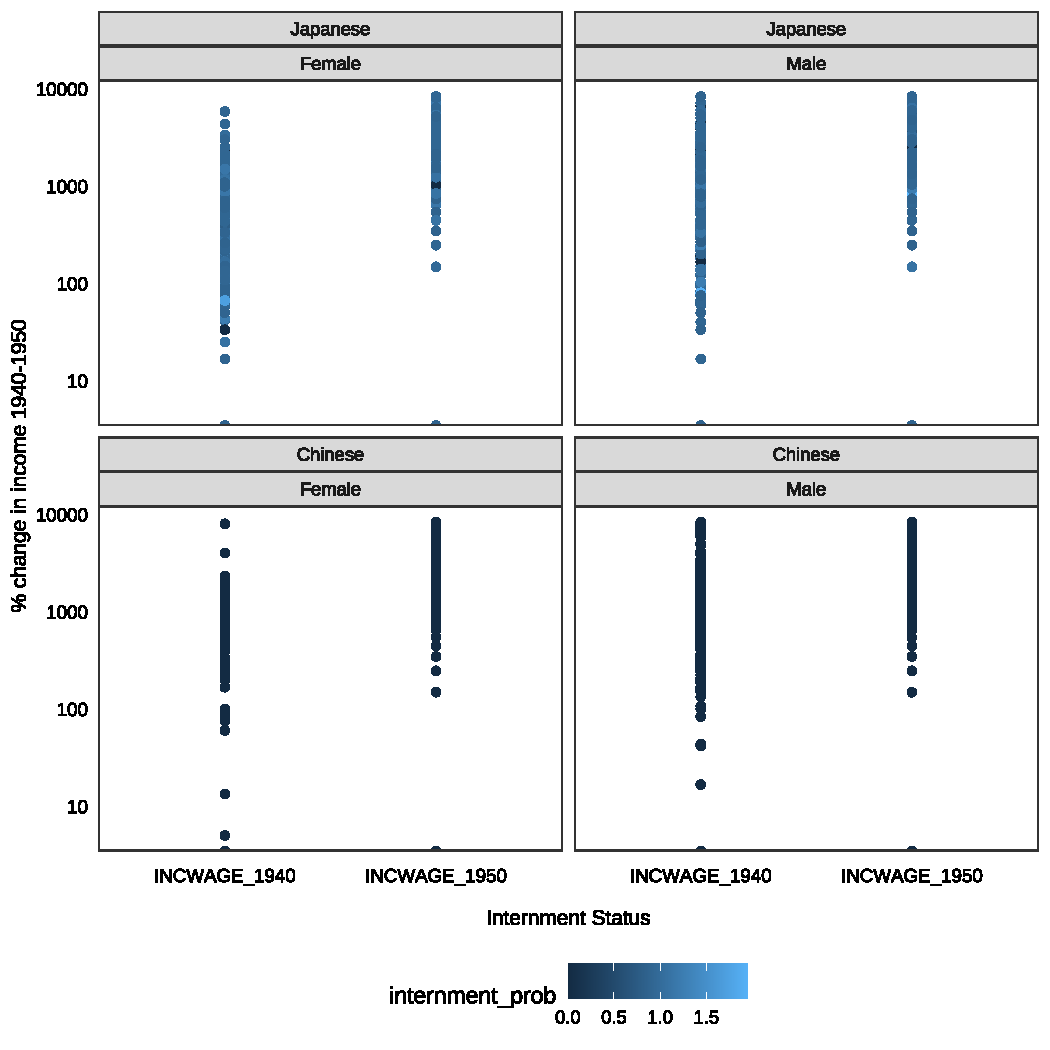
\includegraphics[width=\textwidth]{../figures/INCWAGE_plot.pdf} \\
  \footnotesize
    \emph{Note:}
  Interned proportions are calculated as the number of internees from the county divided by the county's Japanese population in the 1940 full-count census.
  Counties in white had zero Japanese respondents in the 1940 census.
  The map on the below comes from the 1942 Western Defense Command's Final Report 
  % \citep{dewittjohnl.FinalReportJapanese1943}
  and shows in color the evacuation areas along the West Coast.
\end{figure}


Table \ref{tbl:reghet} shows the results of \ref{eq:mainreg}
broken down into separate subsamples.
Without accounting for sex at all in the original sample,
the effect of internment appears negative and statistically insignificant.
Columns (2) and (3) separate out this sample into men and women, respectively.
In the sample with only Japanese and Chinese men,
there does not appear to be a significant effect of internment status on 1950 income.
However, for the sample with Japanese and Chinese women,
this effect is positive and significant at the 1\% level.

\begin{table}[htbp]
   \caption{\label{tbl:reghet} Internment income effect heterogeneities}
   \bigskip
   \centering
   \begin{tabular}{lccccc}
      \toprule
       & \multicolumn{5}{c}{Income in 1950}\\
                                   & All            & Male            & Female         & JM              & JF \\   
                                   & (1)            & (2)             & (3)            & (4)             & (5)\\  
      \midrule 
      Internment Status            & -76.05         & -83.67          & 132.1$^{***}$  & -26.61          & 196.4$^{**}$\\   
                                   & (45.60)        & (66.66)         & (13.65)        & (147.2)         & (71.33)\\   
      Age                          & -17.52$^{***}$ & 39.90$^{***}$   & -43.55$^{***}$ & 65.18$^{***}$   & -41.25$^{***}$\\   
                                   & (4.961)        & (7.969)         & (8.167)        & (9.087)         & (10.80)\\   
      Age square                   & -0.0053        & -0.5879$^{***}$ & 0.2729$^{***}$ & -0.8232$^{***}$ & 0.2289$^{**}$\\   
                                   & (0.0467)       & (0.0771)        & (0.0752)       & (0.0881)        & (0.1026)\\   
      Income in 1940               & 0.3155$^{***}$ & 0.2021$^{***}$  & 0.3344$^{***}$ & 0.1535$^{***}$  & 0.1910$^{***}$\\   
                                   & (0.0158)       & (0.0176)        & (0.0715)       & (0.0140)        & (0.0318)\\   
       \\
      Observations                 & 8,136          & 4,921           & 3,215          & 3,427           & 2,640\\  
      R$^2$                        & 0.08718        & 0.08390         & 0.07804        & 0.08074         & 0.07355\\  
      Within R$^2$                 & 0.05617        & 0.05126         & 0.04222        & 0.04392         & 0.03915\\  
       \\
      Education fixed effects      & $\checkmark$   & $\checkmark$    & $\checkmark$   & $\checkmark$    & $\checkmark$\\   
      State$_{1940}$ fixed effects & $\checkmark$   & $\checkmark$    & $\checkmark$   & $\checkmark$    & $\checkmark$\\   
      \bottomrule
   \end{tabular}
   
   \par \raggedright 
   This table reports the estimates of internment status on 1950 wages across different subsamples of the main linked sample. Column (1) includes Japanese and Chinese men and women, column (2) includes only Japanese and Chinese men, column (3) includes only Japanese and Chinese women, and column (4) includes only Japanese men.
\end{table}

These results seem to suggest that even though my earlier regressions
controlled for sex on the right-hand side,
it may be that internee women were driving the earlier results.
Both Japanese and Chinese women seem to have experienced increases in earnings
over this period.
This is potentially because of increased labor force participation by women
during World War II carrying over into 1950.
Even considering this broad pattern,
Japanese internee women still seem to do better than other women in this sample.

Columns (4) and (5) further restrict the sample to only Japanese men
and Japanese women.
The internment status coefficient for men remains insignificant,
but the coefficient for women is even larger.
Because this sample is smaller than the overall sample,
there are fewer observations with which to estimate the main coefficient.
Despite the lower power, the positive estimated effect for Japanese women remains higher.

If Japanese experienced different levels of discrimination
than Chinese after the war,
then it might be possible that in the regressions
which include them in the control group,
the coefficient on internment status is biased downward.
By including Japanese in columns (4) and (5),
the control group comprises only those Japanese
who lived in counties unaffected by internment
and who would have experienced arguably similar levels of discrimination
to the interned Japanese.
\section{Conclusion}
\label{sec:org2e561ee}

By linking newly available 1940-1950 census data
with War Relocation Authority records,
I constructed a measure of the predicted probability of internment
and compared post-war outcomes for Japanese Americans
against a control group of Chinese Americans.
I sought to answer a puzzle posed by the case of Japanese internment:
how could the forced internment have paradoxically
led to economic opportunity for some?
My results agree with surprising finding that a higher probability of internment
is associated with higher individual earnings in 1950, after resettlement had occurred.
However, this aggregate effect masks a critical source of heterogeneity;
the gains were driven almost entirely by women.
While those likely to be interned were more prone to migrate to higher-income and urban counties,
this channel only partially explains the results.
This could suggest that internment fundamentally altered the labor market trajectories of women
in ways not captured by simple occupational changes.

These findings build on a growing literature
that re-evaluates the long-run economic consequences of internment.
My work aligns with recent studies
by \citet{arellano-boverDisplacementDiversityMobility2022}
and \citet{shoagCausalEffectPlace2016}
in documenting upward mobility,
but it adds a crucial dimension by revealing that these gains were not uniform.
The concentration of effects among women
suggests that the forced break from pre-war community structures
and labor market constraints on the West Coast
may have paradoxically opened new avenues for economic participation in the postwar economy.
Although internees lost their freedoms, property, and dignity,
these results provide a more complex understanding
of how individuals subjected to forced removal
can also adapt to their new environments.

\bibliographystyle{apalike}
\bibliography{internment_refs}
\section{Appendix}
\label{sec:org29d8be6}
\subsection{Figures}
\label{sec:org0c0c087}
\begin{figure}
  \centering
  \caption{Map of Exclusion Area, Assembly Centers, and WRA Camps}
  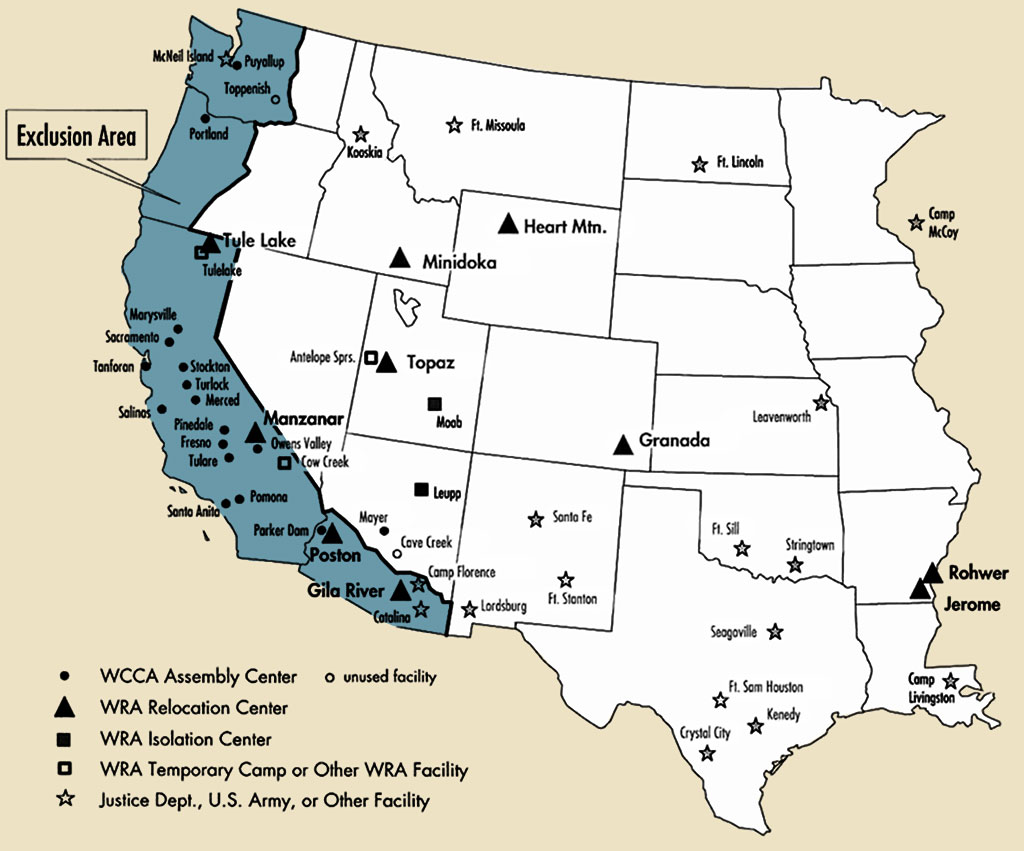
\includegraphics[width=1.0\textwidth]{../figures/PioCrtInternmentMap.jpg}
  \label{fig:internmentmap}
  \caption*{\textit{Source}: \href{https://pioneercourthouse.org/gallery-Japanese-American-Internment.html}{Pioneer Courthouse Galleries}}
\end{figure}

\begin{figure}
  \centering
  \caption{\label{fig:1940JAmap} Map of 1940 Japanese Population Distribution}
  \includegraphics[width=1.0\textwidth]{../figures/1940_map.pdf}
  \caption*{
    \emph{Note:}
    The map shows the numbers of individual census respondents
    in the 1940 full-count census
    whose reported race is Japanese in each county in 1940.
    Color scale is logged to show differences across smaller counties.
    County boundaries come from the 
    \href{https://data2.nhgis.org/}{NHGIS GIS extract system}
    all 1940 US counties excluding Alaska and Hawaii
    using the 2008 TIGER/Line basis.
    Internment camp coordinates come from
    the \href{https://www.arcgis.com/home/item.html?id=69183af8d45d4f46a9dc4eba99440891}{Behind Barbed Wires}
    story map project from the Library of Congress.
  }
\end{figure}

\begin{figure}
  \caption{\label{fig:internee-ages} Counts of interned persons by age and WRA camp}
  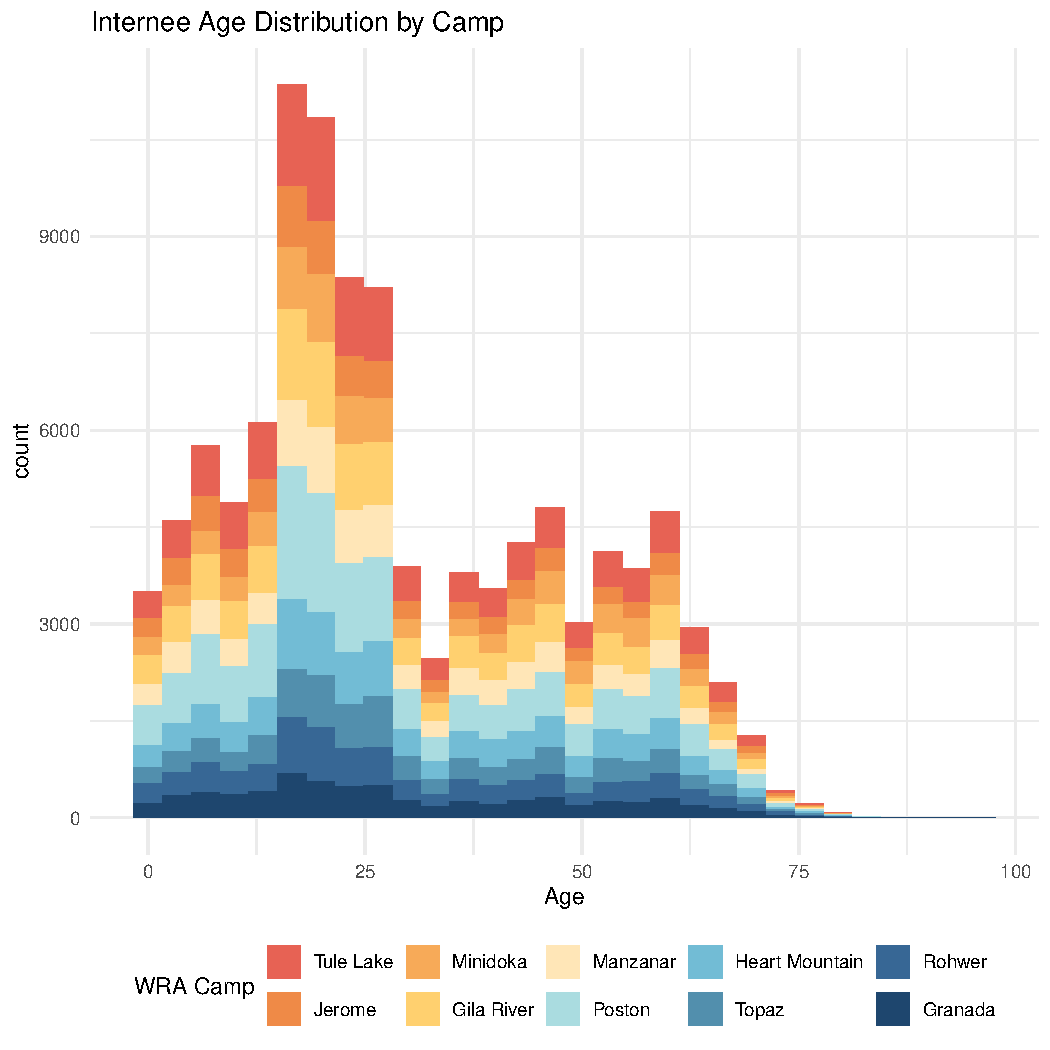
\includegraphics[width=0.6\textwidth]{../figures/internee-age_plot.pdf}
  \footnotesize \\
    \emph{Note:}
  Data from the WRA internment camp records on the ages of interned Japanese people in 1942
  infered from their reported birth year. 
  The counts of people in each of the ten internment camps created by the WRA are based on the initial camp they were placed in 
  after being moved from the temporary assembly centers.
\end{figure}

\begin{figure}
  \caption{\label{fig:pr_intern}Counts of linked individuals by their estimated internment `probability'}
  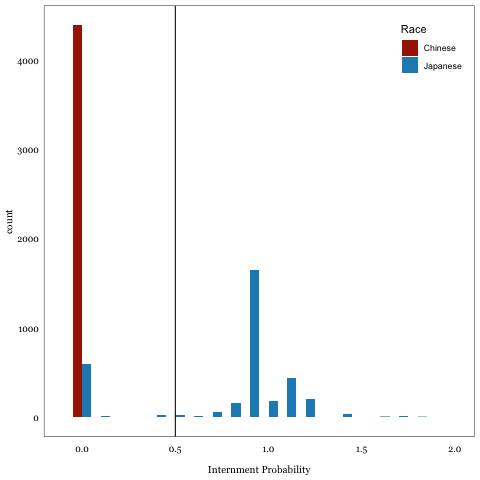
\includegraphics[width=.8\textwidth]{../figures/pr_intern_plot.png} \\
  \footnotesize
    \emph{Note:}
  This figure includes all Japanese and Chinese individuals who are linked across the 1940 and 1950 censuses
  in version 1.2 of the IPUMS MLP project.
  An individual's probability of being an internee is estimated as the ratio of interned people to the 
  number of people in the 1940 full-count census who have the same county and demographics.
  My cutoff for categorizing a person in the linked records as a likely internee is shown by the vertical line at 0.5.
\end{figure}

\begin{table}[ht]
  \caption{\label{tbl:cmp-cty} Top 20 county origins of internees}
  \setlength{\tabcolsep}{4pt}
  \begin{adjustbox}{width=\textwidth, center}
  \begin{tabular}{|ll|r|r|r|r|r|r|r|r|r|r|r|}
    \hline
    state & county & Jer & Manz & Post & Gila & Tule & Mind & Topz & HrtM & Grnd & Rhwr & Total \\ 
    \hline
    CA & L. Angeles & 3049 & 8879 & 2780 & 4851 & 360 &  28 &  62 & 6342 & 2837 & 4331 & 33520 \\ 
    WA & King &  &   1 &   8 &  20 & 2679 & 5852 &   8 &  18 &   6 &   6 & 8598 \\ 
    CA & Sac. & 965 & 376 & 664 & 401 & 4841 &  10 &  19 &   6 & 487 &  58 & 7827 \\ 
    CA & Fresno & 1942 &  25 & 1591 & 1936 &  37 &   8 &  20 &   1 &  23 &  37 & 5620 \\ 
    CA & S. Joaquin &   4 & 160 &  18 & 779 & 356 &  31 &  22 &   3 &  27 & 3511 & 4912 \\ 
    CA & S. Francisco &  59 &  81 &  63 & 174 & 225 &   6 & 3359 & 671 &  74 &  80 & 4792 \\ 
    CA & Alameda &  60 &  20 &  95 & 328 & 300 &  16 & 3635 & 111 &  77 &  51 & 4694 \\ 
    CA & S. Clara &  57 &  16 & 467 & 207 & 219 &  & 134 & 2502 &  50 &  16 & 3669 \\ 
    OR & Multnomah &  &   1 &   1 &  & 308 & 1864 &   1 &  66 &   1 &  & 2242 \\ 
    CA & Tulare & 199 &   4 & 1947 &  25 &   5 &   6 &   9 &   1 &   2 &   4 & 2202 \\ 
    CA & S. Diego &  25 &  38 & 1877 &  17 &   2 &   4 &   1 &  19 &  11 &   3 & 1997 \\ 
    WA & Pierce &  &   3 &  &  & 938 & 999 &  &   4 &  &   2 & 1946 \\ 
    CA & S. Barbara &  38 &  16 &  44 & 1767 &  16 &   1 &   7 &  23 &   6 &  20 & 1938 \\ 
    CA & Orange &  28 &  78 & 1611 &  57 &  10 &  &   3 &  17 &  10 &  41 & 1855 \\ 
    CA & Monterey &  44 &   8 & 1490 &  73 & 125 &   3 &  25 &   7 &  37 &  10 & 1822 \\ 
    CA & Placer &   3 &  &  10 &  & 1746 &   3 &   1 &   1 &   2 &   1 & 1767 \\ 
    CA & Imperial &  &   7 & 1486 &  16 &   2 &  &   2 &  11 &  &   6 & 1530 \\ 
    CA & S. Cruz &  23 &  & 1203 &  46 &  88 &   1 &   1 &  16 &  13 &   7 & 1398 \\ 
    CA & Kern & 332 &  13 & 821 &  16 &   9 &  10 &  10 &   2 &  13 &  15 & 1241 \\ 
    CA & Yolo &   1 &   1 &  10 & 120 & 348 &  &  &  & 626 &  & 1106 \\ 
     \hline
  \end{tabular}
\end{adjustbox}
  \footnotesize
  Numbers represent of count of internees who came from each county who were initially placed in one of the ten WRA camps.
  The camp name abbreviations in the table correspond to Jerome, Manzanar, Poston, Tule Lake, Minidoka, Topaz, Heart Mountain, Granada, and Rohwer.
  The Total column is the sum of all internees from the county across all camps.
\end{table}
\end{document}
